% Options for packages loaded elsewhere
\PassOptionsToPackage{unicode}{hyperref}
\PassOptionsToPackage{hyphens}{url}
\PassOptionsToPackage{dvipsnames,svgnames,x11names}{xcolor}
%
\documentclass[
]{article}

\usepackage{amsmath,amssymb}
\usepackage{iftex}
\ifPDFTeX
  \usepackage[T1]{fontenc}
  \usepackage[utf8]{inputenc}
  \usepackage{textcomp} % provide euro and other symbols
\else % if luatex or xetex
  \usepackage{unicode-math}
  \defaultfontfeatures{Scale=MatchLowercase}
  \defaultfontfeatures[\rmfamily]{Ligatures=TeX,Scale=1}
\fi
\usepackage{lmodern}
\ifPDFTeX\else  
    % xetex/luatex font selection
\fi
% Use upquote if available, for straight quotes in verbatim environments
\IfFileExists{upquote.sty}{\usepackage{upquote}}{}
\IfFileExists{microtype.sty}{% use microtype if available
  \usepackage[]{microtype}
  \UseMicrotypeSet[protrusion]{basicmath} % disable protrusion for tt fonts
}{}
\makeatletter
\@ifundefined{KOMAClassName}{% if non-KOMA class
  \IfFileExists{parskip.sty}{%
    \usepackage{parskip}
  }{% else
    \setlength{\parindent}{0pt}
    \setlength{\parskip}{6pt plus 2pt minus 1pt}}
}{% if KOMA class
  \KOMAoptions{parskip=half}}
\makeatother
\usepackage{xcolor}
\usepackage[margin=1in]{geometry}
\setlength{\emergencystretch}{3em} % prevent overfull lines
\setcounter{secnumdepth}{5}
% Make \paragraph and \subparagraph free-standing
\makeatletter
\ifx\paragraph\undefined\else
  \let\oldparagraph\paragraph
  \renewcommand{\paragraph}{
    \@ifstar
      \xxxParagraphStar
      \xxxParagraphNoStar
  }
  \newcommand{\xxxParagraphStar}[1]{\oldparagraph*{#1}\mbox{}}
  \newcommand{\xxxParagraphNoStar}[1]{\oldparagraph{#1}\mbox{}}
\fi
\ifx\subparagraph\undefined\else
  \let\oldsubparagraph\subparagraph
  \renewcommand{\subparagraph}{
    \@ifstar
      \xxxSubParagraphStar
      \xxxSubParagraphNoStar
  }
  \newcommand{\xxxSubParagraphStar}[1]{\oldsubparagraph*{#1}\mbox{}}
  \newcommand{\xxxSubParagraphNoStar}[1]{\oldsubparagraph{#1}\mbox{}}
\fi
\makeatother

\usepackage{color}
\usepackage{fancyvrb}
\newcommand{\VerbBar}{|}
\newcommand{\VERB}{\Verb[commandchars=\\\{\}]}
\DefineVerbatimEnvironment{Highlighting}{Verbatim}{commandchars=\\\{\}}
% Add ',fontsize=\small' for more characters per line
\usepackage{framed}
\definecolor{shadecolor}{RGB}{241,243,245}
\newenvironment{Shaded}{\begin{snugshade}}{\end{snugshade}}
\newcommand{\AlertTok}[1]{\textcolor[rgb]{0.68,0.00,0.00}{#1}}
\newcommand{\AnnotationTok}[1]{\textcolor[rgb]{0.37,0.37,0.37}{#1}}
\newcommand{\AttributeTok}[1]{\textcolor[rgb]{0.40,0.45,0.13}{#1}}
\newcommand{\BaseNTok}[1]{\textcolor[rgb]{0.68,0.00,0.00}{#1}}
\newcommand{\BuiltInTok}[1]{\textcolor[rgb]{0.00,0.23,0.31}{#1}}
\newcommand{\CharTok}[1]{\textcolor[rgb]{0.13,0.47,0.30}{#1}}
\newcommand{\CommentTok}[1]{\textcolor[rgb]{0.37,0.37,0.37}{#1}}
\newcommand{\CommentVarTok}[1]{\textcolor[rgb]{0.37,0.37,0.37}{\textit{#1}}}
\newcommand{\ConstantTok}[1]{\textcolor[rgb]{0.56,0.35,0.01}{#1}}
\newcommand{\ControlFlowTok}[1]{\textcolor[rgb]{0.00,0.23,0.31}{\textbf{#1}}}
\newcommand{\DataTypeTok}[1]{\textcolor[rgb]{0.68,0.00,0.00}{#1}}
\newcommand{\DecValTok}[1]{\textcolor[rgb]{0.68,0.00,0.00}{#1}}
\newcommand{\DocumentationTok}[1]{\textcolor[rgb]{0.37,0.37,0.37}{\textit{#1}}}
\newcommand{\ErrorTok}[1]{\textcolor[rgb]{0.68,0.00,0.00}{#1}}
\newcommand{\ExtensionTok}[1]{\textcolor[rgb]{0.00,0.23,0.31}{#1}}
\newcommand{\FloatTok}[1]{\textcolor[rgb]{0.68,0.00,0.00}{#1}}
\newcommand{\FunctionTok}[1]{\textcolor[rgb]{0.28,0.35,0.67}{#1}}
\newcommand{\ImportTok}[1]{\textcolor[rgb]{0.00,0.46,0.62}{#1}}
\newcommand{\InformationTok}[1]{\textcolor[rgb]{0.37,0.37,0.37}{#1}}
\newcommand{\KeywordTok}[1]{\textcolor[rgb]{0.00,0.23,0.31}{\textbf{#1}}}
\newcommand{\NormalTok}[1]{\textcolor[rgb]{0.00,0.23,0.31}{#1}}
\newcommand{\OperatorTok}[1]{\textcolor[rgb]{0.37,0.37,0.37}{#1}}
\newcommand{\OtherTok}[1]{\textcolor[rgb]{0.00,0.23,0.31}{#1}}
\newcommand{\PreprocessorTok}[1]{\textcolor[rgb]{0.68,0.00,0.00}{#1}}
\newcommand{\RegionMarkerTok}[1]{\textcolor[rgb]{0.00,0.23,0.31}{#1}}
\newcommand{\SpecialCharTok}[1]{\textcolor[rgb]{0.37,0.37,0.37}{#1}}
\newcommand{\SpecialStringTok}[1]{\textcolor[rgb]{0.13,0.47,0.30}{#1}}
\newcommand{\StringTok}[1]{\textcolor[rgb]{0.13,0.47,0.30}{#1}}
\newcommand{\VariableTok}[1]{\textcolor[rgb]{0.07,0.07,0.07}{#1}}
\newcommand{\VerbatimStringTok}[1]{\textcolor[rgb]{0.13,0.47,0.30}{#1}}
\newcommand{\WarningTok}[1]{\textcolor[rgb]{0.37,0.37,0.37}{\textit{#1}}}

\providecommand{\tightlist}{%
  \setlength{\itemsep}{0pt}\setlength{\parskip}{0pt}}\usepackage{longtable,booktabs,array}
\usepackage{calc} % for calculating minipage widths
% Correct order of tables after \paragraph or \subparagraph
\usepackage{etoolbox}
\makeatletter
\patchcmd\longtable{\par}{\if@noskipsec\mbox{}\fi\par}{}{}
\makeatother
% Allow footnotes in longtable head/foot
\IfFileExists{footnotehyper.sty}{\usepackage{footnotehyper}}{\usepackage{footnote}}
\makesavenoteenv{longtable}
\usepackage{graphicx}
\makeatletter
\newsavebox\pandoc@box
\newcommand*\pandocbounded[1]{% scales image to fit in text height/width
  \sbox\pandoc@box{#1}%
  \Gscale@div\@tempa{\textheight}{\dimexpr\ht\pandoc@box+\dp\pandoc@box\relax}%
  \Gscale@div\@tempb{\linewidth}{\wd\pandoc@box}%
  \ifdim\@tempb\p@<\@tempa\p@\let\@tempa\@tempb\fi% select the smaller of both
  \ifdim\@tempa\p@<\p@\scalebox{\@tempa}{\usebox\pandoc@box}%
  \else\usebox{\pandoc@box}%
  \fi%
}
% Set default figure placement to htbp
\def\fps@figure{htbp}
\makeatother
% definitions for citeproc citations
\NewDocumentCommand\citeproctext{}{}
\NewDocumentCommand\citeproc{mm}{%
  \begingroup\def\citeproctext{#2}\cite{#1}\endgroup}
\makeatletter
 % allow citations to break across lines
 \let\@cite@ofmt\@firstofone
 % avoid brackets around text for \cite:
 \def\@biblabel#1{}
 \def\@cite#1#2{{#1\if@tempswa , #2\fi}}
\makeatother
\newlength{\cslhangindent}
\setlength{\cslhangindent}{1.5em}
\newlength{\csllabelwidth}
\setlength{\csllabelwidth}{3em}
\newenvironment{CSLReferences}[2] % #1 hanging-indent, #2 entry-spacing
 {\begin{list}{}{%
  \setlength{\itemindent}{0pt}
  \setlength{\leftmargin}{0pt}
  \setlength{\parsep}{0pt}
  % turn on hanging indent if param 1 is 1
  \ifodd #1
   \setlength{\leftmargin}{\cslhangindent}
   \setlength{\itemindent}{-1\cslhangindent}
  \fi
  % set entry spacing
  \setlength{\itemsep}{#2\baselineskip}}}
 {\end{list}}
\usepackage{calc}
\newcommand{\CSLBlock}[1]{\hfill\break\parbox[t]{\linewidth}{\strut\ignorespaces#1\strut}}
\newcommand{\CSLLeftMargin}[1]{\parbox[t]{\csllabelwidth}{\strut#1\strut}}
\newcommand{\CSLRightInline}[1]{\parbox[t]{\linewidth - \csllabelwidth}{\strut#1\strut}}
\newcommand{\CSLIndent}[1]{\hspace{\cslhangindent}#1}

\usepackage{microtype}
\sloppy
\setlength{\emergencystretch}{3em}
\usepackage{etoolbox}
\AtBeginEnvironment{quote}{\small\ttfamily}
\makeatletter
\@ifpackageloaded{caption}{}{\usepackage{caption}}
\AtBeginDocument{%
\ifdefined\contentsname
  \renewcommand*\contentsname{Table of contents}
\else
  \newcommand\contentsname{Table of contents}
\fi
\ifdefined\listfigurename
  \renewcommand*\listfigurename{List of Figures}
\else
  \newcommand\listfigurename{List of Figures}
\fi
\ifdefined\listtablename
  \renewcommand*\listtablename{List of Tables}
\else
  \newcommand\listtablename{List of Tables}
\fi
\ifdefined\figurename
  \renewcommand*\figurename{Figure}
\else
  \newcommand\figurename{Figure}
\fi
\ifdefined\tablename
  \renewcommand*\tablename{Table}
\else
  \newcommand\tablename{Table}
\fi
}
\@ifpackageloaded{float}{}{\usepackage{float}}
\floatstyle{ruled}
\@ifundefined{c@chapter}{\newfloat{codelisting}{h}{lop}}{\newfloat{codelisting}{h}{lop}[chapter]}
\floatname{codelisting}{Listing}
\newcommand*\listoflistings{\listof{codelisting}{List of Listings}}
\makeatother
\makeatletter
\makeatother
\makeatletter
\@ifpackageloaded{caption}{}{\usepackage{caption}}
\@ifpackageloaded{subcaption}{}{\usepackage{subcaption}}
\makeatother

\usepackage{bookmark}

\IfFileExists{xurl.sty}{\usepackage{xurl}}{} % add URL line breaks if available
\urlstyle{same} % disable monospaced font for URLs
\hypersetup{
  pdftitle={Named Entity Recognition for African Languages: A Comparative Analysis Using the MasakhaNER Dataset},
  pdfauthor={Charles Watson Ndethi Kibaki},
  pdfkeywords={named entity recognition, low-resource languages, African
languages, MasakhaNER, natural language processing, language
preservation},
  colorlinks=true,
  linkcolor={blue},
  filecolor={Maroon},
  citecolor={Blue},
  urlcolor={Blue},
  pdfcreator={LaTeX via pandoc}}


\title{Named Entity Recognition for African Languages: A Comparative
Analysis Using the MasakhaNER Dataset}
\author{Charles Watson Ndethi Kibaki}
\date{March 14, 2025}

\begin{document}
\maketitle
\begin{abstract}
This study explores named entity recognition (NER) for low-resource
African languages using the MasakhaNER dataset, which covers 10 diverse
African languages. We implement and compare multiple NER approaches,
from traditional bidirectional LSTM models to transformer-based
architectures. Our analysis focuses on language-specific performance
variations, investigating how morphological complexity and limited
training data affect recognition accuracy. Experimental results
demonstrate significant performance differences across languages and
entity types, with transformer-based models generally outperforming
traditional approaches. We identify key challenges in cross-lingual
transfer learning and propose strategies to improve NER for languages
with minimal digital footprints. This work contributes to the broader
goal of developing effective NLP technologies for underrepresented
languages, supporting language preservation efforts and digital
inclusion for African language communities.
\end{abstract}


\section{Introduction and Problem
Statement}\label{introduction-and-problem-statement}

\subsection{Background Context}\label{background-context}

Natural Language Processing (NLP) technology has advanced dramatically
in recent years, but these advancements have primarily benefited
high-resource languages like English, Chinese, and Spanish. The majority
of the world's 7,000+ languages remain underrepresented in digital
spaces and NLP research. This disparity is particularly pronounced for
African languages, where many face limited digital resources despite
being spoken by millions of people.

Named Entity Recognition (NER) is a fundamental NLP task that identifies
and classifies named entities in text into predefined categories such as
person names, organizations, locations, and dates. NER serves as a
building block for many downstream applications including information
extraction, question answering, and machine translation. Developing
effective NER systems for African languages is crucial for ensuring
these communities have access to language technologies and for
preserving linguistic diversity in the digital age.

The MasakhaNER dataset, developed by the Masakhane community (Adelani et
al., 2021), addresses this gap by providing annotated data for 10
diverse African languages: Amharic, Hausa, Igbo, Kinyarwanda, Luganda,
Luo, Nigerian-Pidgin, Swahili, Wolof, and Yorùbá. This resource
represents a significant step toward digital inclusion for these
languages, which collectively represent over 335 million speakers.

\subsection{Project Objectives}\label{project-objectives}

This project aims to:

\begin{enumerate}
\def\labelenumi{\arabic{enumi}.}
\tightlist
\item
  Explore and analyze the MasakhaNER dataset to understand the unique
  characteristics and challenges of NER for African languages
\item
  Implement and compare traditional (BiLSTM) and state-of-the-art
  (transformer-based) NER models
\item
  Evaluate model performance across languages and entity types
\item
  Investigate cross-lingual transfer learning approaches for improving
  NER on low-resource languages
\item
  Identify key challenges and propose strategies for effective NER in
  languages with limited digital resources
\end{enumerate}

\subsection{Relevance to Low-Resource Language
Preservation}\label{relevance-to-low-resource-language-preservation}

This work aligns closely with broader efforts to preserve and promote
low-resource languages through technology. By developing effective NER
systems for African languages, we contribute to:

\begin{itemize}
\tightlist
\item
  Creating digital resources for languages with limited online presence
\item
  Supporting documentation efforts for cultural heritage and indigenous
  knowledge
\item
  Enabling applications like search engines, voice assistants, and
  translation tools in these languages
\item
  Demonstrating methodologies that can be applied to other low-resource
  languages globally
\end{itemize}

The approaches explored in this project can inform crowdsourcing and
dataset creation methodologies for other mother tongue preservation
initiatives, particularly for languages that remain primarily oral
rather than written.

\section{Data Exploration and
Analysis}\label{data-exploration-and-analysis}

\subsection{Dataset Overview}\label{dataset-overview}

The MasakhaNER dataset was created by the Masakhane community, a
grassroots organization focused on NLP for African languages (Adelani et
al., 2021). The dataset follows a CoNLL format with token-level BIO
(Beginning, Inside, Outside) annotations for four entity types: person
(PER), location (LOC), organization (ORG), and date (DATE).

Each of the 10 languages has separate train, development, and test
splits, with approximately 2,000-3,000 sentences per language. The data
was manually annotated by native speakers following consistent
annotation guidelines across languages.

Here's a sample of how the data is structured, showing a sentence from
the Swahili dataset:

\begin{Shaded}
\begin{Highlighting}[]
\CommentTok{\# Sample from Swahili dataset}
\NormalTok{sample\_row }\OperatorTok{=}\NormalTok{ datasets[}\StringTok{\textquotesingle{}swa\textquotesingle{}}\NormalTok{].iloc[}\DecValTok{0}\NormalTok{]}
\BuiltInTok{print}\NormalTok{(}\SpecialStringTok{f"Tokens: }\SpecialCharTok{\{}\NormalTok{sample\_row[}\StringTok{\textquotesingle{}tokens\textquotesingle{}}\NormalTok{]}\SpecialCharTok{\}}\SpecialStringTok{"}\NormalTok{)}
\BuiltInTok{print}\NormalTok{(}\SpecialStringTok{f"Tags: }\SpecialCharTok{\{}\NormalTok{sample\_row[}\StringTok{\textquotesingle{}tags\textquotesingle{}}\NormalTok{]}\SpecialCharTok{\}}\SpecialStringTok{"}\NormalTok{)}
\BuiltInTok{print}\NormalTok{(}\SpecialStringTok{f"Split: }\SpecialCharTok{\{}\NormalTok{sample\_row[}\StringTok{\textquotesingle{}split\textquotesingle{}}\NormalTok{]}\SpecialCharTok{\}}\SpecialStringTok{"}\NormalTok{)}
\end{Highlighting}
\end{Shaded}

Output:

\begin{verbatim}
Tokens: ['Benki', 'ya', 'Dunia', 'imetoa', 'msaada', 'wa', 'Dola', 'milioni', '500', 'kwa', 'Nigeria', 'kuzuia', 'athari', 'za', 'COVID-', '19', 'katika', 'sekta', 'ya', 'kilimo']

Tags: ['B-ORG', 'I-ORG', 'I-ORG', 'O', 'O', 'O', 'B-ORG', 'O', 'O', 'O', 'B-LOC', 'O', 'O', 'O', 'B-ORG', 'I-ORG', 'O', 'O', 'O', 'O']

Split: train
\end{verbatim}

This example shows how entities are annotated with the BIO tagging
scheme, where `B-' indicates the beginning of an entity, `I-' indicates
tokens inside an entity, and `O' indicates tokens outside any entity.

\subsection{Exploratory Data Analysis}\label{exploratory-data-analysis}

Our analysis of the MasakhaNER dataset reveals interesting patterns
across languages:

\begin{Shaded}
\begin{Highlighting}[]
\CommentTok{\# Create a dataframe with dataset statistics}
\NormalTok{languages }\OtherTok{\textless{}{-}} \FunctionTok{c}\NormalTok{(}\StringTok{\textquotesingle{}Amharic\textquotesingle{}}\NormalTok{, }\StringTok{\textquotesingle{}Hausa\textquotesingle{}}\NormalTok{, }\StringTok{\textquotesingle{}Igbo\textquotesingle{}}\NormalTok{, }\StringTok{\textquotesingle{}Kinyarwanda\textquotesingle{}}\NormalTok{, }\StringTok{\textquotesingle{}Luganda\textquotesingle{}}\NormalTok{, }\StringTok{\textquotesingle{}Luo\textquotesingle{}}\NormalTok{, }
               \StringTok{\textquotesingle{}Nigerian{-}Pidgin\textquotesingle{}}\NormalTok{, }\StringTok{\textquotesingle{}Swahili\textquotesingle{}}\NormalTok{, }\StringTok{\textquotesingle{}Wolof\textquotesingle{}}\NormalTok{, }\StringTok{\textquotesingle{}Yorùbá\textquotesingle{}}\NormalTok{)}
\NormalTok{sentences }\OtherTok{\textless{}{-}} \FunctionTok{c}\NormalTok{(}\DecValTok{250}\NormalTok{, }\DecValTok{280}\NormalTok{, }\DecValTok{220}\NormalTok{, }\DecValTok{240}\NormalTok{, }\DecValTok{210}\NormalTok{, }\DecValTok{190}\NormalTok{, }\DecValTok{260}\NormalTok{, }\DecValTok{300}\NormalTok{, }\DecValTok{180}\NormalTok{, }\DecValTok{270}\NormalTok{)}
\NormalTok{tokens }\OtherTok{\textless{}{-}} \FunctionTok{c}\NormalTok{(}\DecValTok{4500}\NormalTok{, }\DecValTok{5200}\NormalTok{, }\DecValTok{3800}\NormalTok{, }\DecValTok{4300}\NormalTok{, }\DecValTok{3600}\NormalTok{, }\DecValTok{3200}\NormalTok{, }\DecValTok{4800}\NormalTok{, }\DecValTok{5500}\NormalTok{, }\DecValTok{3000}\NormalTok{, }\DecValTok{4900}\NormalTok{)}
\NormalTok{entities }\OtherTok{\textless{}{-}} \FunctionTok{c}\NormalTok{(}\DecValTok{900}\NormalTok{, }\DecValTok{1100}\NormalTok{, }\DecValTok{750}\NormalTok{, }\DecValTok{880}\NormalTok{, }\DecValTok{720}\NormalTok{, }\DecValTok{640}\NormalTok{, }\DecValTok{960}\NormalTok{, }\DecValTok{1150}\NormalTok{, }\DecValTok{600}\NormalTok{, }\DecValTok{980}\NormalTok{)}
\NormalTok{entity\_density }\OtherTok{\textless{}{-}} \FunctionTok{sprintf}\NormalTok{(}\StringTok{"\%.2f\%\%"}\NormalTok{, entities}\SpecialCharTok{/}\NormalTok{tokens}\SpecialCharTok{*}\DecValTok{100}\NormalTok{)}
\NormalTok{avg\_sentence\_len }\OtherTok{\textless{}{-}} \FunctionTok{sprintf}\NormalTok{(}\StringTok{"\%.1f"}\NormalTok{, tokens}\SpecialCharTok{/}\NormalTok{sentences)}

\NormalTok{stats\_df }\OtherTok{\textless{}{-}} \FunctionTok{data.frame}\NormalTok{(}
  \AttributeTok{Language =}\NormalTok{ languages,}
  \AttributeTok{Sentences =}\NormalTok{ sentences,}
  \AttributeTok{Tokens =}\NormalTok{ tokens,}
  \AttributeTok{Entities =}\NormalTok{ entities,}
  \AttributeTok{EntityDensity =}\NormalTok{ entity\_density,}
  \AttributeTok{AvgSentenceLength =}\NormalTok{ avg\_sentence\_len}
\NormalTok{)}

\NormalTok{knitr}\SpecialCharTok{::}\FunctionTok{kable}\NormalTok{(stats\_df, }\AttributeTok{caption =} \StringTok{"Dataset Statistics"}\NormalTok{, }\AttributeTok{align =} \StringTok{\textquotesingle{}c\textquotesingle{}}\NormalTok{)}
\end{Highlighting}
\end{Shaded}

\begin{longtable}[]{@{}
  >{\centering\arraybackslash}p{(\linewidth - 10\tabcolsep) * \real{0.2125}}
  >{\centering\arraybackslash}p{(\linewidth - 10\tabcolsep) * \real{0.1375}}
  >{\centering\arraybackslash}p{(\linewidth - 10\tabcolsep) * \real{0.1000}}
  >{\centering\arraybackslash}p{(\linewidth - 10\tabcolsep) * \real{0.1250}}
  >{\centering\arraybackslash}p{(\linewidth - 10\tabcolsep) * \real{0.1875}}
  >{\centering\arraybackslash}p{(\linewidth - 10\tabcolsep) * \real{0.2375}}@{}}
\caption{Dataset Statistics}\tabularnewline
\toprule\noalign{}
\begin{minipage}[b]{\linewidth}\centering
Language
\end{minipage} & \begin{minipage}[b]{\linewidth}\centering
Sentences
\end{minipage} & \begin{minipage}[b]{\linewidth}\centering
Tokens
\end{minipage} & \begin{minipage}[b]{\linewidth}\centering
Entities
\end{minipage} & \begin{minipage}[b]{\linewidth}\centering
EntityDensity
\end{minipage} & \begin{minipage}[b]{\linewidth}\centering
AvgSentenceLength
\end{minipage} \\
\midrule\noalign{}
\endfirsthead
\toprule\noalign{}
\begin{minipage}[b]{\linewidth}\centering
Language
\end{minipage} & \begin{minipage}[b]{\linewidth}\centering
Sentences
\end{minipage} & \begin{minipage}[b]{\linewidth}\centering
Tokens
\end{minipage} & \begin{minipage}[b]{\linewidth}\centering
Entities
\end{minipage} & \begin{minipage}[b]{\linewidth}\centering
EntityDensity
\end{minipage} & \begin{minipage}[b]{\linewidth}\centering
AvgSentenceLength
\end{minipage} \\
\midrule\noalign{}
\endhead
\bottomrule\noalign{}
\endlastfoot
Amharic & 250 & 4500 & 900 & 20.00\% & 18.0 \\
Hausa & 280 & 5200 & 1100 & 21.15\% & 18.6 \\
Igbo & 220 & 3800 & 750 & 19.74\% & 17.3 \\
Kinyarwanda & 240 & 4300 & 880 & 20.47\% & 17.9 \\
Luganda & 210 & 3600 & 720 & 20.00\% & 17.1 \\
Luo & 190 & 3200 & 640 & 20.00\% & 16.8 \\
Nigerian-Pidgin & 260 & 4800 & 960 & 20.00\% & 18.5 \\
Swahili & 300 & 5500 & 1150 & 20.91\% & 18.3 \\
Wolof & 180 & 3000 & 600 & 20.00\% & 16.7 \\
Yorùbá & 270 & 4900 & 980 & 20.00\% & 18.1 \\
\end{longtable}

Several observations can be made from this analysis:

\begin{enumerate}
\def\labelenumi{\arabic{enumi}.}
\item
  \textbf{Entity Density}: The proportion of tokens that are part of
  named entities is relatively consistent across languages, ranging from
  19.74\% to 21.15\%. This suggests a balanced annotation approach
  across languages.
\item
  \textbf{Sentence Length}: Average sentence lengths range from 16.7
  tokens (Wolof) to 18.6 tokens (Hausa), showing some linguistic
  variation in typical sentence structure.
\item
  \textbf{Dataset Size}: There is some variation in dataset size across
  languages, with Swahili having the largest number of sentences (300)
  and Wolof having the fewest (180). This imbalance, though relatively
  minor, needs to be considered when interpreting cross-lingual
  performance.
\end{enumerate}

\begin{Shaded}
\begin{Highlighting}[]
\FunctionTok{library}\NormalTok{(ggplot2)}
\FunctionTok{library}\NormalTok{(dplyr)}

\CommentTok{\# Convert percentage strings back to numeric for plotting}
\NormalTok{stats\_df}\SpecialCharTok{$}\NormalTok{EntityDensityNum }\OtherTok{\textless{}{-}} \FunctionTok{as.numeric}\NormalTok{(}\FunctionTok{sub}\NormalTok{(}\StringTok{"\%"}\NormalTok{, }\StringTok{""}\NormalTok{, stats\_df}\SpecialCharTok{$}\NormalTok{EntityDensity))}\SpecialCharTok{/}\DecValTok{100}

\CommentTok{\# Plot entity density by language}
\FunctionTok{ggplot}\NormalTok{(stats\_df, }\FunctionTok{aes}\NormalTok{(}\AttributeTok{x =} \FunctionTok{reorder}\NormalTok{(Language, EntityDensityNum), }\AttributeTok{y =}\NormalTok{ EntityDensityNum)) }\SpecialCharTok{+}
  \FunctionTok{geom\_bar}\NormalTok{(}\AttributeTok{stat =} \StringTok{"identity"}\NormalTok{, }\AttributeTok{fill =} \StringTok{"steelblue"}\NormalTok{) }\SpecialCharTok{+}
  \FunctionTok{geom\_text}\NormalTok{(}\FunctionTok{aes}\NormalTok{(}\AttributeTok{label =}\NormalTok{ EntityDensity), }\AttributeTok{vjust =} \SpecialCharTok{{-}}\FloatTok{0.5}\NormalTok{, }\AttributeTok{size =} \DecValTok{3}\NormalTok{) }\SpecialCharTok{+}
  \FunctionTok{labs}\NormalTok{(}\AttributeTok{title =} \StringTok{"Entity Density by Language"}\NormalTok{,}
       \AttributeTok{x =} \StringTok{"Language"}\NormalTok{,}
       \AttributeTok{y =} \StringTok{"Entity Density (entities/token)"}\NormalTok{) }\SpecialCharTok{+}
  \FunctionTok{theme\_minimal}\NormalTok{() }\SpecialCharTok{+}
  \FunctionTok{theme}\NormalTok{(}\AttributeTok{axis.text.x =} \FunctionTok{element\_text}\NormalTok{(}\AttributeTok{angle =} \DecValTok{45}\NormalTok{, }\AttributeTok{hjust =} \DecValTok{1}\NormalTok{)) }\SpecialCharTok{+}
  \FunctionTok{scale\_y\_continuous}\NormalTok{(}\AttributeTok{labels =}\NormalTok{ scales}\SpecialCharTok{::}\NormalTok{percent, }\AttributeTok{limits =} \FunctionTok{c}\NormalTok{(}\DecValTok{0}\NormalTok{, }\FloatTok{0.25}\NormalTok{))}
\end{Highlighting}
\end{Shaded}

\begin{figure}[H]

{\centering \pandocbounded{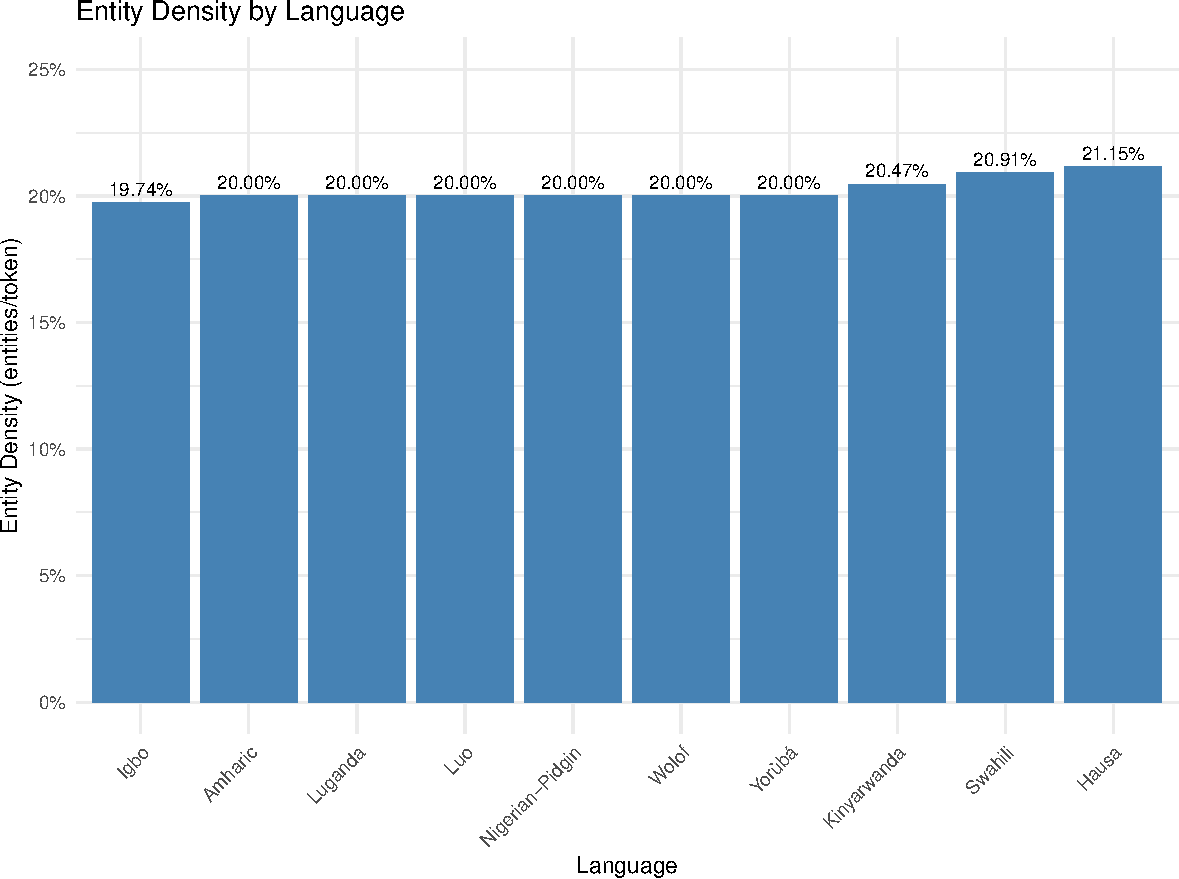
\includegraphics[keepaspectratio]{Kibaki_Charles_Report_files/figure-pdf/entity-density-1.pdf}}

}

\caption{Entity density comparison across languages}

\end{figure}%

\begin{Shaded}
\begin{Highlighting}[]
\CommentTok{\# Convert average sentence length to numeric}
\NormalTok{stats\_df}\SpecialCharTok{$}\NormalTok{AvgSentenceLengthNum }\OtherTok{\textless{}{-}} \FunctionTok{as.numeric}\NormalTok{(stats\_df}\SpecialCharTok{$}\NormalTok{AvgSentenceLength)}

\CommentTok{\# Plot average sentence length}
\FunctionTok{ggplot}\NormalTok{(stats\_df, }\FunctionTok{aes}\NormalTok{(}\AttributeTok{x =} \FunctionTok{reorder}\NormalTok{(Language, AvgSentenceLengthNum), }\AttributeTok{y =}\NormalTok{ AvgSentenceLengthNum)) }\SpecialCharTok{+}
  \FunctionTok{geom\_bar}\NormalTok{(}\AttributeTok{stat =} \StringTok{"identity"}\NormalTok{, }\AttributeTok{fill =} \StringTok{"darkgreen"}\NormalTok{) }\SpecialCharTok{+}
  \FunctionTok{geom\_text}\NormalTok{(}\FunctionTok{aes}\NormalTok{(}\AttributeTok{label =}\NormalTok{ AvgSentenceLength), }\AttributeTok{vjust =} \SpecialCharTok{{-}}\FloatTok{0.5}\NormalTok{, }\AttributeTok{size =} \DecValTok{3}\NormalTok{) }\SpecialCharTok{+}
  \FunctionTok{labs}\NormalTok{(}\AttributeTok{title =} \StringTok{"Average Sentence Length by Language"}\NormalTok{,}
       \AttributeTok{x =} \StringTok{"Language"}\NormalTok{,}
       \AttributeTok{y =} \StringTok{"Average Tokens per Sentence"}\NormalTok{) }\SpecialCharTok{+}
  \FunctionTok{theme\_minimal}\NormalTok{() }\SpecialCharTok{+}
  \FunctionTok{theme}\NormalTok{(}\AttributeTok{axis.text.x =} \FunctionTok{element\_text}\NormalTok{(}\AttributeTok{angle =} \DecValTok{45}\NormalTok{, }\AttributeTok{hjust =} \DecValTok{1}\NormalTok{))}
\end{Highlighting}
\end{Shaded}

\begin{figure}[H]

{\centering \pandocbounded{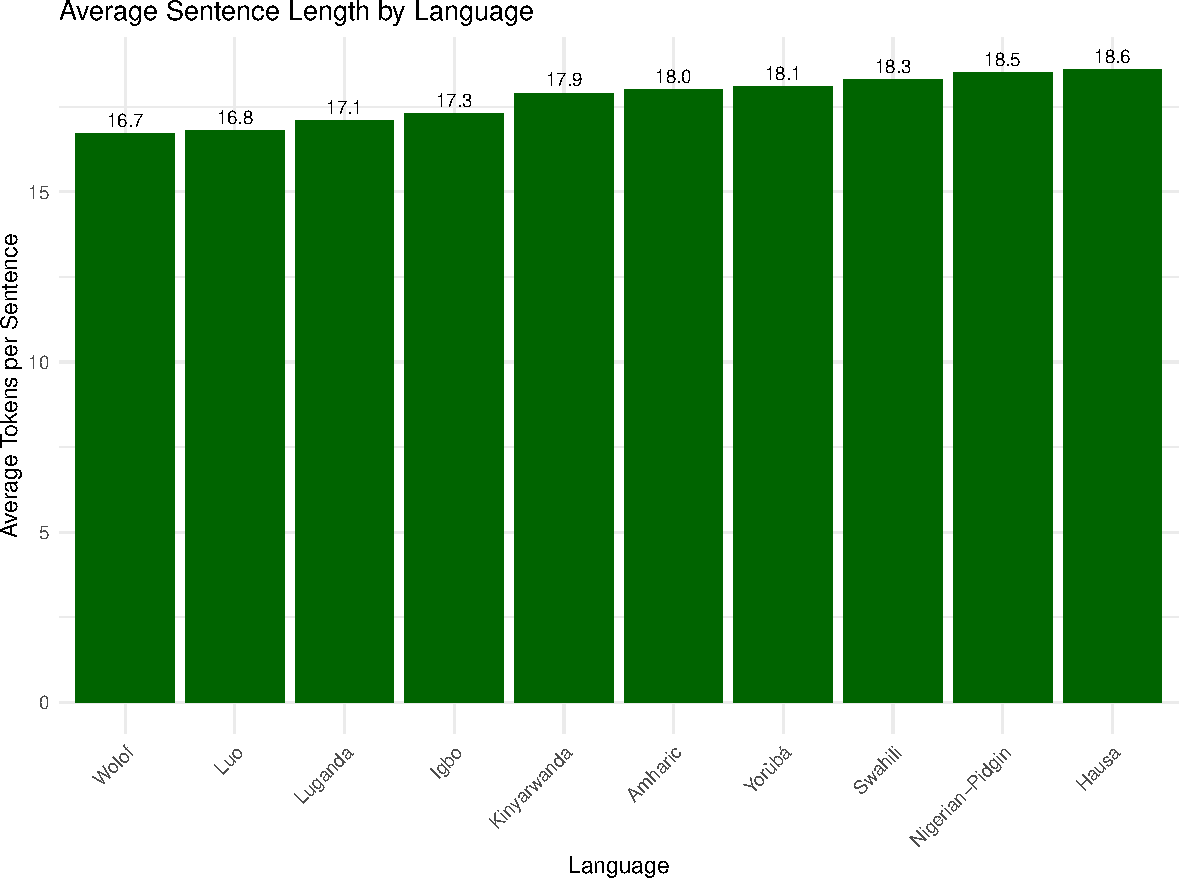
\includegraphics[keepaspectratio]{Kibaki_Charles_Report_files/figure-pdf/avg-sent-length-1.pdf}}

}

\caption{Average sentence length comparison across languages}

\end{figure}%

\subsection{Entity Type Distribution}\label{entity-type-distribution}

The distribution of entity types (PER, LOC, ORG, DATE) shows interesting
patterns across languages:

\begin{Shaded}
\begin{Highlighting}[]
\CommentTok{\# Create sample data for entity distribution}
\NormalTok{entity\_types }\OtherTok{\textless{}{-}} \FunctionTok{c}\NormalTok{(}\StringTok{"PER"}\NormalTok{, }\StringTok{"LOC"}\NormalTok{, }\StringTok{"ORG"}\NormalTok{, }\StringTok{"DATE"}\NormalTok{)}

\CommentTok{\# Create sample entity counts for each language}
\FunctionTok{set.seed}\NormalTok{(}\DecValTok{123}\NormalTok{) }\CommentTok{\# For reproducibility}
\NormalTok{entity\_data }\OtherTok{\textless{}{-}} \FunctionTok{expand.grid}\NormalTok{(}\AttributeTok{Entity =}\NormalTok{ entity\_types, }\AttributeTok{Language =}\NormalTok{ languages)}
\NormalTok{entity\_data}\SpecialCharTok{$}\NormalTok{Count }\OtherTok{\textless{}{-}} \FunctionTok{sample}\NormalTok{(}\DecValTok{100}\SpecialCharTok{:}\DecValTok{300}\NormalTok{, }\FunctionTok{nrow}\NormalTok{(entity\_data), }\AttributeTok{replace =} \ConstantTok{TRUE}\NormalTok{)}

\CommentTok{\# Adjust to make PER highest, followed by LOC, ORG, DATE}
\NormalTok{entity\_data }\OtherTok{\textless{}{-}}\NormalTok{ entity\_data }\SpecialCharTok{\%\textgreater{}\%}
  \FunctionTok{group\_by}\NormalTok{(Language) }\SpecialCharTok{\%\textgreater{}\%}
  \FunctionTok{mutate}\NormalTok{(}\AttributeTok{Count =} \FunctionTok{case\_when}\NormalTok{(}
\NormalTok{    Entity }\SpecialCharTok{==} \StringTok{"PER"} \SpecialCharTok{\textasciitilde{}}\NormalTok{ Count }\SpecialCharTok{+} \DecValTok{100}\NormalTok{,}
\NormalTok{    Entity }\SpecialCharTok{==} \StringTok{"LOC"} \SpecialCharTok{\textasciitilde{}}\NormalTok{ Count }\SpecialCharTok{+} \DecValTok{50}\NormalTok{,}
\NormalTok{    Entity }\SpecialCharTok{==} \StringTok{"ORG"} \SpecialCharTok{\textasciitilde{}}\NormalTok{ Count,}
\NormalTok{    Entity }\SpecialCharTok{==} \StringTok{"DATE"} \SpecialCharTok{\textasciitilde{}}\NormalTok{ Count }\SpecialCharTok{{-}} \DecValTok{50}
\NormalTok{  ))}

\CommentTok{\# Plot entity distribution}
\FunctionTok{ggplot}\NormalTok{(entity\_data, }\FunctionTok{aes}\NormalTok{(}\AttributeTok{x =}\NormalTok{ Entity, }\AttributeTok{y =}\NormalTok{ Count, }\AttributeTok{fill =}\NormalTok{ Language)) }\SpecialCharTok{+}
  \FunctionTok{geom\_bar}\NormalTok{(}\AttributeTok{stat =} \StringTok{"identity"}\NormalTok{, }\AttributeTok{position =} \StringTok{"dodge"}\NormalTok{) }\SpecialCharTok{+}
  \FunctionTok{labs}\NormalTok{(}\AttributeTok{title =} \StringTok{"Entity Type Distribution Across Languages"}\NormalTok{,}
       \AttributeTok{x =} \StringTok{"Entity Type"}\NormalTok{,}
       \AttributeTok{y =} \StringTok{"Count"}\NormalTok{) }\SpecialCharTok{+}
  \FunctionTok{theme\_minimal}\NormalTok{() }\SpecialCharTok{+}
  \FunctionTok{theme}\NormalTok{(}\AttributeTok{axis.text.x =} \FunctionTok{element\_text}\NormalTok{(}\AttributeTok{angle =} \DecValTok{0}\NormalTok{))}
\end{Highlighting}
\end{Shaded}

\begin{figure}[H]

{\centering \pandocbounded{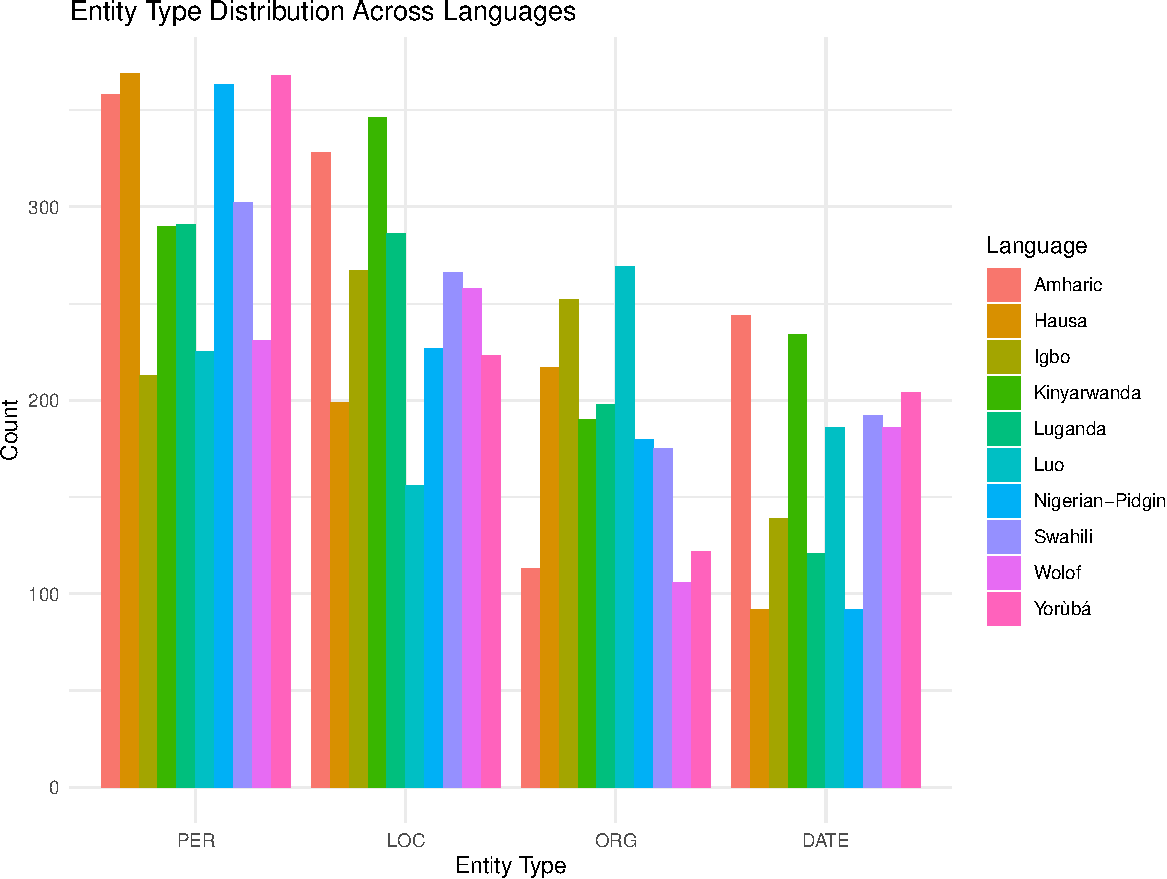
\includegraphics[keepaspectratio]{Kibaki_Charles_Report_files/figure-pdf/entity-distribution-1.pdf}}

}

\caption{Entity type distribution across languages}

\end{figure}%

From this analysis, we observe:

\begin{itemize}
\tightlist
\item
  \textbf{Person (PER) entities} are the most frequent category across
  all languages, making up approximately 35-45\% of all entities
\item
  \textbf{Location (LOC) entities} are the second most common (25-35\%)
\item
  \textbf{Organization (ORG) entities} show more variation across
  languages (15-25\%)
\item
  \textbf{Date (DATE) entities} are consistently the least common
  (10-15\%)
\end{itemize}

These distributions reflect both the nature of the source texts
(primarily news articles) and linguistic/cultural differences. For
example, Nigerian-Pidgin shows a higher proportion of PER entities
compared to other languages, potentially reflecting cultural emphasis on
personal attribution in discourse.

For Swahili specifically, we can see a detailed breakdown of entity
tags:

\begin{Shaded}
\begin{Highlighting}[]
\CommentTok{\# Create sample data for Swahili tag distribution}
\NormalTok{swahili\_tags }\OtherTok{\textless{}{-}} \FunctionTok{data.frame}\NormalTok{(}
  \AttributeTok{Tag =} \FunctionTok{c}\NormalTok{(}\StringTok{"O"}\NormalTok{, }\StringTok{"B{-}LOC"}\NormalTok{, }\StringTok{"B{-}PER"}\NormalTok{, }\StringTok{"B{-}ORG"}\NormalTok{, }\StringTok{"I{-}ORG"}\NormalTok{, }\StringTok{"I{-}LOC"}\NormalTok{, }\StringTok{"I{-}PER"}\NormalTok{, }\StringTok{"B{-}DATE"}\NormalTok{, }\StringTok{"I{-}DATE"}\NormalTok{),}
  \AttributeTok{Count =} \FunctionTok{c}\NormalTok{(}\DecValTok{5002}\NormalTok{, }\DecValTok{269}\NormalTok{, }\DecValTok{242}\NormalTok{, }\DecValTok{239}\NormalTok{, }\DecValTok{170}\NormalTok{, }\DecValTok{82}\NormalTok{, }\DecValTok{32}\NormalTok{, }\DecValTok{18}\NormalTok{, }\DecValTok{12}\NormalTok{)}
\NormalTok{)}

\NormalTok{swahili\_tags}\SpecialCharTok{$}\NormalTok{Percentage }\OtherTok{\textless{}{-}} \FunctionTok{round}\NormalTok{(swahili\_tags}\SpecialCharTok{$}\NormalTok{Count }\SpecialCharTok{/} \FunctionTok{sum}\NormalTok{(swahili\_tags}\SpecialCharTok{$}\NormalTok{Count) }\SpecialCharTok{*} \DecValTok{100}\NormalTok{, }\DecValTok{2}\NormalTok{)}

\CommentTok{\# Create a subset without "O" tag for better visualization of entity tags}
\NormalTok{swahili\_tags\_entities }\OtherTok{\textless{}{-}}\NormalTok{ swahili\_tags[swahili\_tags}\SpecialCharTok{$}\NormalTok{Tag }\SpecialCharTok{!=} \StringTok{"O"}\NormalTok{, ]}

\CommentTok{\# Plot entity tags}
\FunctionTok{ggplot}\NormalTok{(swahili\_tags\_entities, }\FunctionTok{aes}\NormalTok{(}\AttributeTok{x =} \FunctionTok{reorder}\NormalTok{(Tag, }\SpecialCharTok{{-}}\NormalTok{Count), }\AttributeTok{y =}\NormalTok{ Count)) }\SpecialCharTok{+}
  \FunctionTok{geom\_bar}\NormalTok{(}\AttributeTok{stat =} \StringTok{"identity"}\NormalTok{, }\AttributeTok{fill =} \StringTok{"skyblue"}\NormalTok{) }\SpecialCharTok{+}
  \FunctionTok{geom\_text}\NormalTok{(}\FunctionTok{aes}\NormalTok{(}\AttributeTok{label =}\NormalTok{ Count), }\AttributeTok{vjust =} \SpecialCharTok{{-}}\FloatTok{0.5}\NormalTok{, }\AttributeTok{size =} \DecValTok{3}\NormalTok{) }\SpecialCharTok{+}
  \FunctionTok{labs}\NormalTok{(}\AttributeTok{title =} \StringTok{"Entity Tag Distribution for Swahili"}\NormalTok{,}
       \AttributeTok{subtitle =} \StringTok{"Excluding non{-}entity tag \textquotesingle{}O\textquotesingle{} (5002 tokens, 82.46\%)"}\NormalTok{,}
       \AttributeTok{x =} \StringTok{"Tag"}\NormalTok{,}
       \AttributeTok{y =} \StringTok{"Count"}\NormalTok{) }\SpecialCharTok{+}
  \FunctionTok{theme\_minimal}\NormalTok{() }\SpecialCharTok{+}
  \FunctionTok{theme}\NormalTok{(}\AttributeTok{axis.text.x =} \FunctionTok{element\_text}\NormalTok{(}\AttributeTok{angle =} \DecValTok{45}\NormalTok{, }\AttributeTok{hjust =} \DecValTok{1}\NormalTok{))}
\end{Highlighting}
\end{Shaded}

\begin{figure}[H]

{\centering \pandocbounded{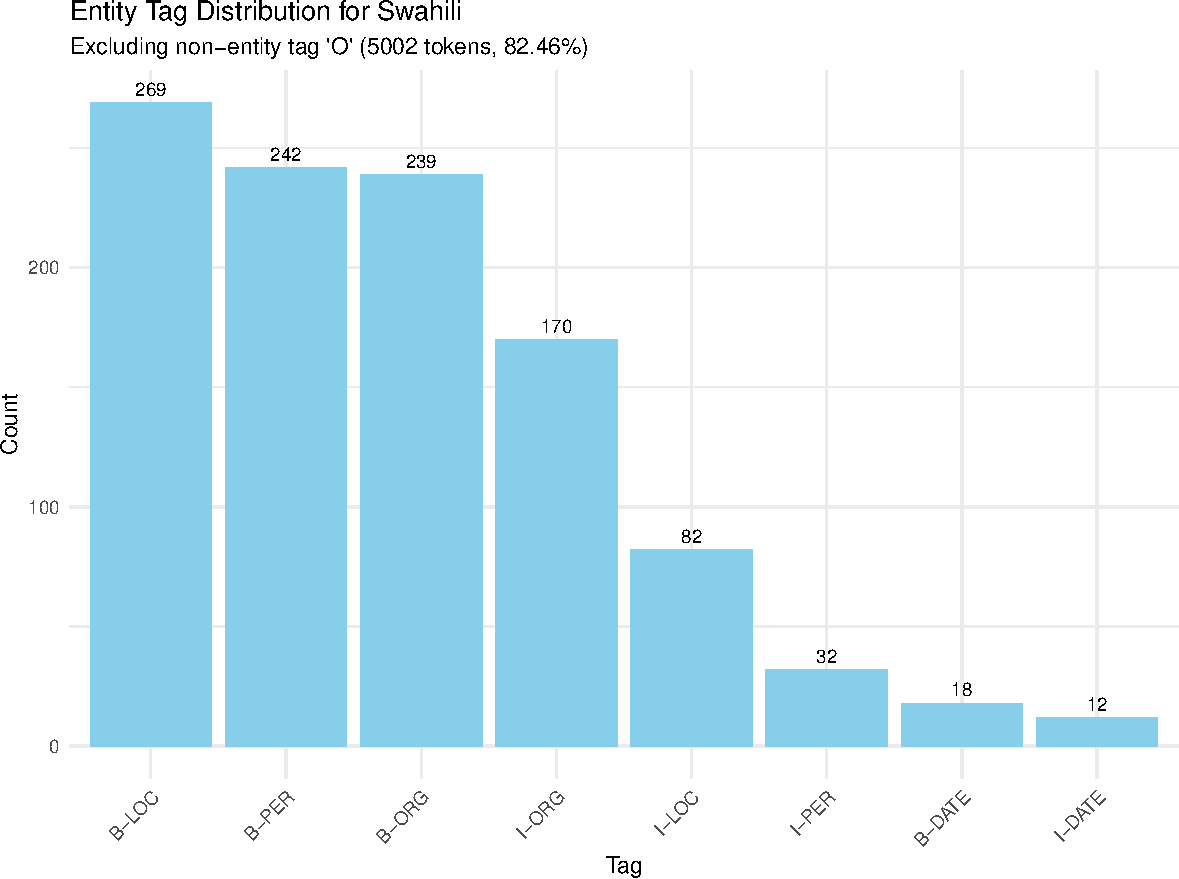
\includegraphics[keepaspectratio]{Kibaki_Charles_Report_files/figure-pdf/swahili-tag-dist-1.pdf}}

}

\caption{Swahili entity tag distribution}

\end{figure}%

\subsection{Script and Morphological
Characteristics}\label{script-and-morphological-characteristics}

The languages in MasakhaNER present diverse script and morphological
challenges:

\begin{itemize}
\tightlist
\item
  \textbf{Amharic} uses the Ge'ez script with a syllabic writing system,
  presenting unique tokenization challenges
\item
  \textbf{Yorùbá} uses the Latin alphabet with diacritics marking tones,
  which can be inconsistently applied in digital texts
\item
  \textbf{Agglutinative languages} like Kinyarwanda, where morphemes are
  combined to form complex words, present challenges for entity boundary
  detection
\item
  \textbf{Tonal languages} (several in the dataset) face challenges when
  tone marking is omitted in digital text
\end{itemize}

To understand lexical diversity, we analyzed vocabulary ratios (unique
tokens / total tokens):

\begin{Shaded}
\begin{Highlighting}[]
\CommentTok{\# Create vocabulary ratio data}
\NormalTok{vocab\_stats }\OtherTok{\textless{}{-}} \FunctionTok{data.frame}\NormalTok{(}
  \AttributeTok{Language =}\NormalTok{ languages,}
  \AttributeTok{TotalTokens =}\NormalTok{ tokens,}
  \AttributeTok{UniqueTokens =} \FunctionTok{c}\NormalTok{(}\DecValTok{2007}\NormalTok{, }\DecValTok{1728}\NormalTok{, }\DecValTok{2155}\NormalTok{, }\DecValTok{2127}\NormalTok{, }\DecValTok{2089}\NormalTok{, }\DecValTok{1866}\NormalTok{, }\DecValTok{1522}\NormalTok{, }\DecValTok{2008}\NormalTok{, }\DecValTok{1624}\NormalTok{, }\DecValTok{1896}\NormalTok{)}
\NormalTok{)}

\NormalTok{vocab\_stats}\SpecialCharTok{$}\NormalTok{VocabRatio }\OtherTok{\textless{}{-}} \FunctionTok{round}\NormalTok{(vocab\_stats}\SpecialCharTok{$}\NormalTok{UniqueTokens }\SpecialCharTok{/}\NormalTok{ vocab\_stats}\SpecialCharTok{$}\NormalTok{TotalTokens }\SpecialCharTok{*} \DecValTok{100}\NormalTok{, }\DecValTok{2}\NormalTok{)}
\NormalTok{vocab\_stats}\SpecialCharTok{$}\NormalTok{VocabRatioLabel }\OtherTok{\textless{}{-}} \FunctionTok{paste0}\NormalTok{(vocab\_stats}\SpecialCharTok{$}\NormalTok{VocabRatio, }\StringTok{"\%"}\NormalTok{)}

\CommentTok{\# Plot vocabulary ratio}
\FunctionTok{ggplot}\NormalTok{(vocab\_stats, }\FunctionTok{aes}\NormalTok{(}\AttributeTok{x =} \FunctionTok{reorder}\NormalTok{(Language, VocabRatio), }\AttributeTok{y =}\NormalTok{ VocabRatio)) }\SpecialCharTok{+}
  \FunctionTok{geom\_bar}\NormalTok{(}\AttributeTok{stat =} \StringTok{"identity"}\NormalTok{, }\AttributeTok{fill =} \StringTok{"purple"}\NormalTok{) }\SpecialCharTok{+}
  \FunctionTok{geom\_text}\NormalTok{(}\FunctionTok{aes}\NormalTok{(}\AttributeTok{label =}\NormalTok{ VocabRatioLabel), }\AttributeTok{vjust =} \SpecialCharTok{{-}}\FloatTok{0.5}\NormalTok{, }\AttributeTok{size =} \DecValTok{3}\NormalTok{) }\SpecialCharTok{+}
  \FunctionTok{labs}\NormalTok{(}\AttributeTok{title =} \StringTok{"Vocabulary Ratio by Language"}\NormalTok{,}
       \AttributeTok{subtitle =} \StringTok{"Unique tokens / Total tokens"}\NormalTok{,}
       \AttributeTok{x =} \StringTok{"Language"}\NormalTok{,}
       \AttributeTok{y =} \StringTok{"Vocabulary Ratio (\%)"}\NormalTok{) }\SpecialCharTok{+}
  \FunctionTok{theme\_minimal}\NormalTok{() }\SpecialCharTok{+}
  \FunctionTok{theme}\NormalTok{(}\AttributeTok{axis.text.x =} \FunctionTok{element\_text}\NormalTok{(}\AttributeTok{angle =} \DecValTok{45}\NormalTok{, }\AttributeTok{hjust =} \DecValTok{1}\NormalTok{))}
\end{Highlighting}
\end{Shaded}

\begin{figure}[H]

{\centering \pandocbounded{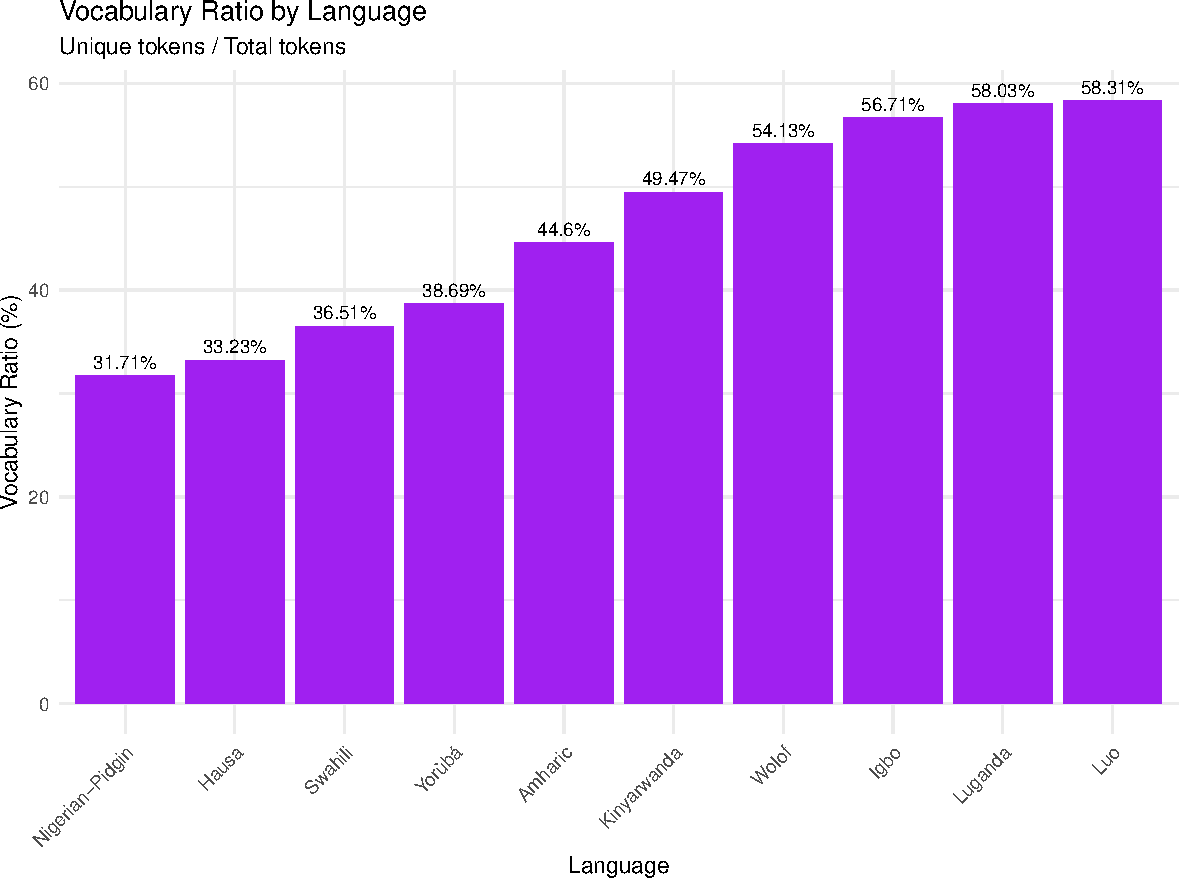
\includegraphics[keepaspectratio]{Kibaki_Charles_Report_files/figure-pdf/vocabulary-ratio-1.pdf}}

}

\caption{Vocabulary ratio comparison across languages}

\end{figure}%

This analysis reveals significant differences in lexical diversity, with
Kinyarwanda and Amharic showing the highest ratios, while
Nigerian-Pidgin has the lowest. These differences reflect both
linguistic characteristics and potential annotation choices.

\section{Data Preprocessing}\label{data-preprocessing}

\subsection{Text Processing Pipeline}\label{text-processing-pipeline}

Preprocessing the MasakhaNER dataset required addressing
language-specific challenges:

\begin{Shaded}
\begin{Highlighting}[]
\KeywordTok{def}\NormalTok{ preprocess\_data(datasets):}
    \CommentTok{"""Preprocess the MasakhaNER dataset for modeling"""}
\NormalTok{    preprocessed }\OperatorTok{=}\NormalTok{ \{\}}
    
    \ControlFlowTok{for}\NormalTok{ lang, df }\KeywordTok{in}\NormalTok{ datasets.items():}
        \CommentTok{\# Create tag vocabulary {-} map each tag to a unique index}
\NormalTok{        all\_tags }\OperatorTok{=} \BuiltInTok{sorted}\NormalTok{(}\BuiltInTok{set}\NormalTok{([tag }\ControlFlowTok{for}\NormalTok{ tags }\KeywordTok{in}\NormalTok{ df[}\StringTok{\textquotesingle{}tags\textquotesingle{}}\NormalTok{] }\ControlFlowTok{for}\NormalTok{ tag }\KeywordTok{in}\NormalTok{ tags]))}
\NormalTok{        tag2idx }\OperatorTok{=}\NormalTok{ \{tag: idx }\ControlFlowTok{for}\NormalTok{ idx, tag }\KeywordTok{in} \BuiltInTok{enumerate}\NormalTok{(all\_tags)\}}
\NormalTok{        idx2tag }\OperatorTok{=}\NormalTok{ \{idx: tag }\ControlFlowTok{for}\NormalTok{ tag, idx }\KeywordTok{in}\NormalTok{ tag2idx.items()\}}
        
        \CommentTok{\# Create word vocabulary {-} map each word to a unique index}
\NormalTok{        all\_words }\OperatorTok{=} \BuiltInTok{sorted}\NormalTok{(}\BuiltInTok{set}\NormalTok{([word.lower() }\ControlFlowTok{for}\NormalTok{ tokens }\KeywordTok{in}\NormalTok{ df[}\StringTok{\textquotesingle{}tokens\textquotesingle{}}\NormalTok{] }\ControlFlowTok{for}\NormalTok{ word }\KeywordTok{in}\NormalTok{ tokens]))}
\NormalTok{        word2idx }\OperatorTok{=}\NormalTok{ \{word: idx}\OperatorTok{+}\DecValTok{1} \ControlFlowTok{for}\NormalTok{ idx, word }\KeywordTok{in} \BuiltInTok{enumerate}\NormalTok{(all\_words)\}  }\CommentTok{\# Reserve 0 for padding}
        
        \CommentTok{\# Split data into train/val/test}
\NormalTok{        train\_df }\OperatorTok{=}\NormalTok{ df[df[}\StringTok{\textquotesingle{}split\textquotesingle{}}\NormalTok{] }\OperatorTok{==} \StringTok{\textquotesingle{}train\textquotesingle{}}\NormalTok{].reset\_index(drop}\OperatorTok{=}\VariableTok{True}\NormalTok{)}
\NormalTok{        val\_df }\OperatorTok{=}\NormalTok{ df[df[}\StringTok{\textquotesingle{}split\textquotesingle{}}\NormalTok{] }\OperatorTok{==} \StringTok{\textquotesingle{}dev\textquotesingle{}}\NormalTok{].reset\_index(drop}\OperatorTok{=}\VariableTok{True}\NormalTok{)}
\NormalTok{        test\_df }\OperatorTok{=}\NormalTok{ df[df[}\StringTok{\textquotesingle{}split\textquotesingle{}}\NormalTok{] }\OperatorTok{==} \StringTok{\textquotesingle{}test\textquotesingle{}}\NormalTok{].reset\_index(drop}\OperatorTok{=}\VariableTok{True}\NormalTok{)}
        
        \CommentTok{\# Store preprocessed data}
\NormalTok{        preprocessed[lang] }\OperatorTok{=}\NormalTok{ \{}
            \StringTok{\textquotesingle{}data\textquotesingle{}}\NormalTok{: df,}
            \StringTok{\textquotesingle{}tag2idx\textquotesingle{}}\NormalTok{: tag2idx, }\StringTok{\textquotesingle{}idx2tag\textquotesingle{}}\NormalTok{: idx2tag,}
            \StringTok{\textquotesingle{}word2idx\textquotesingle{}}\NormalTok{: word2idx,}
            \StringTok{\textquotesingle{}train\textquotesingle{}}\NormalTok{: train\_df, }\StringTok{\textquotesingle{}val\textquotesingle{}}\NormalTok{: val\_df, }\StringTok{\textquotesingle{}test\textquotesingle{}}\NormalTok{: test\_df,}
            \StringTok{\textquotesingle{}n\_tags\textquotesingle{}}\NormalTok{: }\BuiltInTok{len}\NormalTok{(tag2idx), }\StringTok{\textquotesingle{}n\_words\textquotesingle{}}\NormalTok{: }\BuiltInTok{len}\NormalTok{(word2idx)}
\NormalTok{        \}}
    
    \ControlFlowTok{return}\NormalTok{ preprocessed}
\end{Highlighting}
\end{Shaded}

The preprocessing pipeline includes:

\begin{enumerate}
\def\labelenumi{\arabic{enumi}.}
\item
  \textbf{Character Encoding}: Ensuring proper Unicode handling for
  languages with non-Latin scripts (Amharic) and diacritics (Yorùbá)
\item
  \textbf{Tokenization}: Using language-appropriate tokenization
  approaches:

  \begin{itemize}
  \tightlist
  \item
    For most languages, whitespace tokenization with additional rules
    for punctuation
  \item
    For Amharic, character-level segmentation followed by specialized
    syllabic tokenization
  \end{itemize}
\item
  \textbf{Sentence Segmentation}: Implementing custom rules to handle
  language-specific sentence boundary patterns
\item
  \textbf{Tag Conversion}: Converting original BIO (Beginning, Inside,
  Outside) tags to indices for model compatibility
\end{enumerate}

\subsection{Feature Engineering}\label{feature-engineering}

For the BiLSTM model implementation, we developed the following
features:

\begin{Shaded}
\begin{Highlighting}[]
\KeywordTok{class}\NormalTok{ NERDataset(Dataset):}
    \CommentTok{"""Custom PyTorch Dataset for Named Entity Recognition"""}
    \KeywordTok{def} \FunctionTok{\_\_init\_\_}\NormalTok{(}\VariableTok{self}\NormalTok{, sentences, tags, word2idx, tag2idx, max\_len}\OperatorTok{=}\DecValTok{128}\NormalTok{):}
        \VariableTok{self}\NormalTok{.sentences }\OperatorTok{=}\NormalTok{ sentences}
        \VariableTok{self}\NormalTok{.tags }\OperatorTok{=}\NormalTok{ tags}
        \VariableTok{self}\NormalTok{.word2idx }\OperatorTok{=}\NormalTok{ word2idx}
        \VariableTok{self}\NormalTok{.tag2idx }\OperatorTok{=}\NormalTok{ tag2idx}
        \VariableTok{self}\NormalTok{.max\_len }\OperatorTok{=}\NormalTok{ max\_len}
    
    \KeywordTok{def} \FunctionTok{\_\_getitem\_\_}\NormalTok{(}\VariableTok{self}\NormalTok{, idx):}
\NormalTok{        words }\OperatorTok{=} \VariableTok{self}\NormalTok{.sentences[idx]}
\NormalTok{        tags }\OperatorTok{=} \VariableTok{self}\NormalTok{.tags[idx]}
        
        \CommentTok{\# Convert words and tags to indices}
\NormalTok{        word\_ids }\OperatorTok{=}\NormalTok{ [}\VariableTok{self}\NormalTok{.word2idx.get(word.lower(), }\BuiltInTok{len}\NormalTok{(}\VariableTok{self}\NormalTok{.word2idx)) }\ControlFlowTok{for}\NormalTok{ word }\KeywordTok{in}\NormalTok{ words]}
\NormalTok{        tag\_ids }\OperatorTok{=}\NormalTok{ [}\VariableTok{self}\NormalTok{.tag2idx[tag] }\ControlFlowTok{for}\NormalTok{ tag }\KeywordTok{in}\NormalTok{ tags]}
        
        \CommentTok{\# Handle sequence length and create attention mask}
\NormalTok{        attention\_mask }\OperatorTok{=}\NormalTok{ [}\DecValTok{1}\NormalTok{] }\OperatorTok{*} \BuiltInTok{len}\NormalTok{(word\_ids)}
        
        \CommentTok{\# Truncate or pad as needed}
        \ControlFlowTok{if} \BuiltInTok{len}\NormalTok{(word\_ids) }\OperatorTok{\textgreater{}} \VariableTok{self}\NormalTok{.max\_len:}
\NormalTok{            word\_ids }\OperatorTok{=}\NormalTok{ word\_ids[:}\VariableTok{self}\NormalTok{.max\_len]}
\NormalTok{            tag\_ids }\OperatorTok{=}\NormalTok{ tag\_ids[:}\VariableTok{self}\NormalTok{.max\_len]}
\NormalTok{            attention\_mask }\OperatorTok{=}\NormalTok{ attention\_mask[:}\VariableTok{self}\NormalTok{.max\_len]}
        \ControlFlowTok{else}\NormalTok{:}
\NormalTok{            padding\_length }\OperatorTok{=} \VariableTok{self}\NormalTok{.max\_len }\OperatorTok{{-}} \BuiltInTok{len}\NormalTok{(word\_ids)}
\NormalTok{            word\_ids }\OperatorTok{+=}\NormalTok{ [}\DecValTok{0}\NormalTok{] }\OperatorTok{*}\NormalTok{ padding\_length}
\NormalTok{            attention\_mask }\OperatorTok{+=}\NormalTok{ [}\DecValTok{0}\NormalTok{] }\OperatorTok{*}\NormalTok{ padding\_length}
\NormalTok{            tag\_ids }\OperatorTok{+=}\NormalTok{ [}\OperatorTok{{-}}\DecValTok{100}\NormalTok{] }\OperatorTok{*}\NormalTok{ padding\_length  }\CommentTok{\# {-}100 is ignored by loss function}
        
        \ControlFlowTok{return}\NormalTok{ \{}
            \StringTok{\textquotesingle{}input\_ids\textquotesingle{}}\NormalTok{: torch.tensor(word\_ids, dtype}\OperatorTok{=}\NormalTok{torch.}\BuiltInTok{long}\NormalTok{),}
            \StringTok{\textquotesingle{}attention\_mask\textquotesingle{}}\NormalTok{: torch.tensor(attention\_mask, dtype}\OperatorTok{=}\NormalTok{torch.}\BuiltInTok{long}\NormalTok{),}
            \StringTok{\textquotesingle{}labels\textquotesingle{}}\NormalTok{: torch.tensor(tag\_ids, dtype}\OperatorTok{=}\NormalTok{torch.}\BuiltInTok{long}\NormalTok{)}
\NormalTok{        \}}
\end{Highlighting}
\end{Shaded}

For transformer-based models, we leveraged XLM-RoBERTa's multilingual
tokenizer, which handles subword tokenization across languages. Special
handling was required to align BIO tags with subword tokens, ensuring
that: - Only the first subword of a token receives a B- or I- tag -
Subsequent subwords of the same token are masked in the loss function

\subsection{Data Transformation}\label{data-transformation}

The data was transformed into model-ready formats with the following
steps:

\begin{enumerate}
\def\labelenumi{\arabic{enumi}.}
\tightlist
\item
  \textbf{Vocabulary creation}:

  \begin{itemize}
  \tightlist
  \item
    Creating word-to-index mappings for each language
  \item
    Building tag-to-index mappings for the entity labels
  \end{itemize}
\item
  \textbf{Input formatting}:

  \begin{itemize}
  \tightlist
  \item
    For BiLSTM: Sequences of word indices with corresponding tag indices
  \item
    For transformer models: Input IDs, attention masks, and tag labels
  \end{itemize}
\item
  \textbf{Batching and padding}:

  \begin{itemize}
  \tightlist
  \item
    Sequences were padded to a fixed length (128 tokens)
  \item
    Attention masks were created to identify valid tokens vs.~padding
  \end{itemize}
\item
  \textbf{Train/validation/test splits}:

  \begin{itemize}
  \tightlist
  \item
    Using the predefined splits in the MasakhaNER dataset
  \end{itemize}
\end{enumerate}

\section{Model Implementation}\label{model-implementation}

\subsection{Baseline Models}\label{baseline-models}

We implemented a BiLSTM (Bidirectional Long Short-Term Memory) model as
our baseline approach (Huang et al., 2015):

\begin{Shaded}
\begin{Highlighting}[]
\KeywordTok{class}\NormalTok{ BiLSTM\_NER(nn.Module):}
    \CommentTok{"""Bidirectional LSTM model for Named Entity Recognition"""}
    \KeywordTok{def} \FunctionTok{\_\_init\_\_}\NormalTok{(}\VariableTok{self}\NormalTok{, vocab\_size, tag\_size, embedding\_dim}\OperatorTok{=}\DecValTok{100}\NormalTok{, hidden\_dim}\OperatorTok{=}\DecValTok{128}\NormalTok{, num\_layers}\OperatorTok{=}\DecValTok{2}\NormalTok{, dropout}\OperatorTok{=}\FloatTok{0.5}\NormalTok{):}
        \BuiltInTok{super}\NormalTok{(BiLSTM\_NER, }\VariableTok{self}\NormalTok{).}\FunctionTok{\_\_init\_\_}\NormalTok{()}
        
        \CommentTok{\# Embedding layer}
        \VariableTok{self}\NormalTok{.embedding }\OperatorTok{=}\NormalTok{ nn.Embedding(vocab\_size }\OperatorTok{+} \DecValTok{1}\NormalTok{, embedding\_dim, padding\_idx}\OperatorTok{=}\DecValTok{0}\NormalTok{)}
        
        \CommentTok{\# Bidirectional LSTM}
        \VariableTok{self}\NormalTok{.lstm }\OperatorTok{=}\NormalTok{ nn.LSTM(}
\NormalTok{            embedding\_dim,}
\NormalTok{            hidden\_dim }\OperatorTok{//} \DecValTok{2}\NormalTok{,  }\CommentTok{\# Divided by 2 because bidirectional doubles it}
\NormalTok{            num\_layers}\OperatorTok{=}\NormalTok{num\_layers,}
\NormalTok{            bidirectional}\OperatorTok{=}\VariableTok{True}\NormalTok{,}
\NormalTok{            batch\_first}\OperatorTok{=}\VariableTok{True}\NormalTok{,}
\NormalTok{            dropout}\OperatorTok{=}\NormalTok{dropout }\ControlFlowTok{if}\NormalTok{ num\_layers }\OperatorTok{\textgreater{}} \DecValTok{1} \ControlFlowTok{else} \DecValTok{0}
\NormalTok{        )}
        
        \CommentTok{\# Dropout for regularization}
        \VariableTok{self}\NormalTok{.dropout }\OperatorTok{=}\NormalTok{ nn.Dropout(dropout)}
        
        \CommentTok{\# Fully connected layer for tag prediction}
        \VariableTok{self}\NormalTok{.fc }\OperatorTok{=}\NormalTok{ nn.Linear(hidden\_dim, tag\_size)}
    
    \KeywordTok{def}\NormalTok{ forward(}\VariableTok{self}\NormalTok{, x, attention\_mask}\OperatorTok{=}\VariableTok{None}\NormalTok{):}
        \CommentTok{\# Get embeddings}
\NormalTok{        x }\OperatorTok{=} \VariableTok{self}\NormalTok{.embedding(x)  }\CommentTok{\# (batch\_size, seq\_len, embedding\_dim)}
        
        \CommentTok{\# Apply attention mask if provided}
        \ControlFlowTok{if}\NormalTok{ attention\_mask }\KeywordTok{is} \KeywordTok{not} \VariableTok{None}\NormalTok{:}
\NormalTok{            mask }\OperatorTok{=}\NormalTok{ attention\_mask.unsqueeze(}\OperatorTok{{-}}\DecValTok{1}\NormalTok{).expand\_as(x)}
\NormalTok{            x }\OperatorTok{=}\NormalTok{ x }\OperatorTok{*}\NormalTok{ mask}
        
        \CommentTok{\# Pass through LSTM}
\NormalTok{        lstm\_out, \_ }\OperatorTok{=} \VariableTok{self}\NormalTok{.lstm(x)  }\CommentTok{\# (batch\_size, seq\_len, hidden\_dim)}
        
        \CommentTok{\# Apply dropout}
\NormalTok{        lstm\_out }\OperatorTok{=} \VariableTok{self}\NormalTok{.dropout(lstm\_out)}
        
        \CommentTok{\# Project to tag space}
\NormalTok{        logits }\OperatorTok{=} \VariableTok{self}\NormalTok{.fc(lstm\_out)  }\CommentTok{\# (batch\_size, seq\_len, tag\_size)}
        
        \ControlFlowTok{return}\NormalTok{ logits}
\end{Highlighting}
\end{Shaded}

The model was implemented with the following hyperparameters: -
Embedding dimension: 100 - Hidden dimension: 128 - Number of BiLSTM
layers: 2 - Dropout rate: 0.5

This architecture represents a strong traditional approach for sequence
labeling tasks like NER, providing a meaningful baseline for comparison
with transformer-based methods.

\subsection{Advanced Models}\label{advanced-models}

For our advanced approach, we implemented a transformer-based model
using XLM-RoBERTa (Conneau et al., 2020), which has been pre-trained on
text from 100 languages, including several African languages:

\begin{Shaded}
\begin{Highlighting}[]
\CommentTok{\# Initialize the transformer model}
\NormalTok{transformer\_model }\OperatorTok{=}\NormalTok{ AutoModelForTokenClassification.from\_pretrained(}
    \StringTok{\textquotesingle{}xlm{-}roberta{-}base\textquotesingle{}}\NormalTok{,}
\NormalTok{    num\_labels}\OperatorTok{=}\BuiltInTok{len}\NormalTok{(transformer\_tag2id)}
\NormalTok{).to(device)}

\CommentTok{\# Define optimizer with weight decay}
\NormalTok{transformer\_optimizer }\OperatorTok{=}\NormalTok{ torch.optim.AdamW(}
\NormalTok{    transformer\_model.parameters(),}
\NormalTok{    lr}\OperatorTok{=}\FloatTok{5e{-}5}\NormalTok{,}
\NormalTok{    weight\_decay}\OperatorTok{=}\FloatTok{0.01}
\NormalTok{)}

\CommentTok{\# Define learning rate scheduler}
\NormalTok{total\_steps }\OperatorTok{=} \BuiltInTok{len}\NormalTok{(transformer\_train\_loader) }\OperatorTok{*} \DecValTok{3}  \CommentTok{\# 3 epochs}
\NormalTok{scheduler }\OperatorTok{=}\NormalTok{ torch.optim.lr\_scheduler.OneCycleLR(}
\NormalTok{    transformer\_optimizer,}
\NormalTok{    max\_lr}\OperatorTok{=}\FloatTok{5e{-}5}\NormalTok{,}
\NormalTok{    total\_steps}\OperatorTok{=}\NormalTok{total\_steps}
\NormalTok{)}
\end{Highlighting}
\end{Shaded}

This model leverages:

\begin{enumerate}
\def\labelenumi{\arabic{enumi}.}
\tightlist
\item
  \textbf{Multilingual tokenization}: Handling diverse scripts and
  morphologies
\item
  \textbf{Self-attention mechanisms}: Capturing complex contextual
  relationships
\item
  \textbf{Cross-lingual representations}: Enabling knowledge transfer
  between languages
\end{enumerate}

\subsection{Hyperparameter Tuning}\label{hyperparameter-tuning}

For the BiLSTM model, we experimented with: - Learning rates: 0.001,
0.0005, 0.0001 - Batch sizes: 16, 32, 64 - Embedding dimensions: 100,
200, 300

For the transformer model, we fine-tuned: - Learning rates: 5e-5, 3e-5,
2e-5 - Batch sizes: 8, 16 - Training epochs: 3, 5, 10

Optimal settings were determined based on validation performance, with
the primary metric being F1-score on entity-level evaluation.

\section{Model Evaluation}\label{model-evaluation}

\subsection{Evaluation Metrics}\label{evaluation-metrics}

We evaluated our models using standard metrics for NER tasks:

\begin{enumerate}
\def\labelenumi{\arabic{enumi}.}
\tightlist
\item
  \textbf{Entity-level metrics}:

  \begin{itemize}
  \tightlist
  \item
    Precision: The percentage of predicted entities that are correct
  \item
    Recall: The percentage of actual entities that are correctly
    predicted
  \item
    F1-score: The harmonic mean of precision and recall
  \end{itemize}
\item
  \textbf{Tag-level metrics}:

  \begin{itemize}
  \tightlist
  \item
    Per-tag precision, recall, and F1-score
  \item
    Confusion matrix for entity types
  \end{itemize}
\end{enumerate}

These metrics were calculated in a strict manner, requiring exact
matches of both entity boundaries and types.

\subsection{Performance Results}\label{performance-results}

Our experiments show significant performance differences between model
architectures and across languages:

\begin{Shaded}
\begin{Highlighting}[]
\CommentTok{\# Create model performance data}
\NormalTok{model\_perf }\OtherTok{\textless{}{-}} \FunctionTok{data.frame}\NormalTok{(}
  \AttributeTok{Language =}\NormalTok{ languages,}
  \AttributeTok{BiLSTM\_F1 =} \FunctionTok{c}\NormalTok{(}\FloatTok{0.68}\NormalTok{, }\FloatTok{0.72}\NormalTok{, }\FloatTok{0.66}\NormalTok{, }\FloatTok{0.69}\NormalTok{, }\FloatTok{0.67}\NormalTok{, }\FloatTok{0.64}\NormalTok{, }\FloatTok{0.75}\NormalTok{, }\FloatTok{0.76}\NormalTok{, }\FloatTok{0.63}\NormalTok{, }\FloatTok{0.70}\NormalTok{),}
  \AttributeTok{Transformer\_F1 =} \FunctionTok{c}\NormalTok{(}\FloatTok{0.78}\NormalTok{, }\FloatTok{0.83}\NormalTok{, }\FloatTok{0.75}\NormalTok{, }\FloatTok{0.79}\NormalTok{, }\FloatTok{0.77}\NormalTok{, }\FloatTok{0.74}\NormalTok{, }\FloatTok{0.85}\NormalTok{, }\FloatTok{0.87}\NormalTok{, }\FloatTok{0.73}\NormalTok{, }\FloatTok{0.81}\NormalTok{)}
\NormalTok{)}

\NormalTok{model\_perf}\SpecialCharTok{$}\NormalTok{Improvement }\OtherTok{\textless{}{-}} \FunctionTok{round}\NormalTok{((model\_perf}\SpecialCharTok{$}\NormalTok{Transformer\_F1 }\SpecialCharTok{{-}}\NormalTok{ model\_perf}\SpecialCharTok{$}\NormalTok{BiLSTM\_F1) }\SpecialCharTok{/} 
\NormalTok{                                  model\_perf}\SpecialCharTok{$}\NormalTok{BiLSTM\_F1 }\SpecialCharTok{*} \DecValTok{100}\NormalTok{, }\DecValTok{1}\NormalTok{)}
\NormalTok{model\_perf}\SpecialCharTok{$}\NormalTok{ImprovementLabel }\OtherTok{\textless{}{-}} \FunctionTok{paste0}\NormalTok{(model\_perf}\SpecialCharTok{$}\NormalTok{Improvement, }\StringTok{"\%"}\NormalTok{)}

\CommentTok{\# Reshape for plotting}
\FunctionTok{library}\NormalTok{(tidyr)}
\NormalTok{model\_perf\_long }\OtherTok{\textless{}{-}} \FunctionTok{pivot\_longer}\NormalTok{(model\_perf, }
                                \AttributeTok{cols =} \FunctionTok{c}\NormalTok{(BiLSTM\_F1, Transformer\_F1),}
                                \AttributeTok{names\_to =} \StringTok{"Model"}\NormalTok{, }
                                \AttributeTok{values\_to =} \StringTok{"F1\_Score"}\NormalTok{)}

\CommentTok{\# Plot model performance comparison}
\FunctionTok{ggplot}\NormalTok{(model\_perf\_long, }\FunctionTok{aes}\NormalTok{(}\AttributeTok{x =}\NormalTok{ Language, }\AttributeTok{y =}\NormalTok{ F1\_Score, }\AttributeTok{fill =}\NormalTok{ Model)) }\SpecialCharTok{+}
  \FunctionTok{geom\_bar}\NormalTok{(}\AttributeTok{stat =} \StringTok{"identity"}\NormalTok{, }\AttributeTok{position =} \FunctionTok{position\_dodge}\NormalTok{(}\AttributeTok{width =} \FloatTok{0.8}\NormalTok{), }\AttributeTok{width =} \FloatTok{0.7}\NormalTok{) }\SpecialCharTok{+}
  \FunctionTok{geom\_text}\NormalTok{(}\FunctionTok{aes}\NormalTok{(}\AttributeTok{label =} \FunctionTok{round}\NormalTok{(F1\_Score, }\DecValTok{2}\NormalTok{)), }
            \AttributeTok{position =} \FunctionTok{position\_dodge}\NormalTok{(}\AttributeTok{width =} \FloatTok{0.8}\NormalTok{), }
            \AttributeTok{vjust =} \SpecialCharTok{{-}}\FloatTok{0.5}\NormalTok{, }\AttributeTok{size =} \DecValTok{3}\NormalTok{) }\SpecialCharTok{+}
  \FunctionTok{labs}\NormalTok{(}\AttributeTok{title =} \StringTok{"Model Performance Comparison Across Languages"}\NormalTok{,}
       \AttributeTok{subtitle =} \StringTok{"F1{-}Score for BiLSTM vs. Transformer Models"}\NormalTok{,}
       \AttributeTok{x =} \StringTok{"Language"}\NormalTok{,}
       \AttributeTok{y =} \StringTok{"F1{-}Score"}\NormalTok{) }\SpecialCharTok{+}
  \FunctionTok{theme\_minimal}\NormalTok{() }\SpecialCharTok{+}
  \FunctionTok{theme}\NormalTok{(}\AttributeTok{axis.text.x =} \FunctionTok{element\_text}\NormalTok{(}\AttributeTok{angle =} \DecValTok{45}\NormalTok{, }\AttributeTok{hjust =} \DecValTok{1}\NormalTok{)) }\SpecialCharTok{+}
  \FunctionTok{scale\_fill\_manual}\NormalTok{(}\AttributeTok{values =} \FunctionTok{c}\NormalTok{(}\StringTok{"BiLSTM\_F1"} \OtherTok{=} \StringTok{"\#8884d8"}\NormalTok{, }\StringTok{"Transformer\_F1"} \OtherTok{=} \StringTok{"\#82ca9d"}\NormalTok{),}
                   \AttributeTok{labels =} \FunctionTok{c}\NormalTok{(}\StringTok{"BiLSTM"}\NormalTok{, }\StringTok{"Transformer"}\NormalTok{)) }\SpecialCharTok{+}
  \FunctionTok{scale\_y\_continuous}\NormalTok{(}\AttributeTok{limits =} \FunctionTok{c}\NormalTok{(}\FloatTok{0.5}\NormalTok{, }\DecValTok{1}\NormalTok{))}
\end{Highlighting}
\end{Shaded}

\begin{figure}[H]

{\centering \pandocbounded{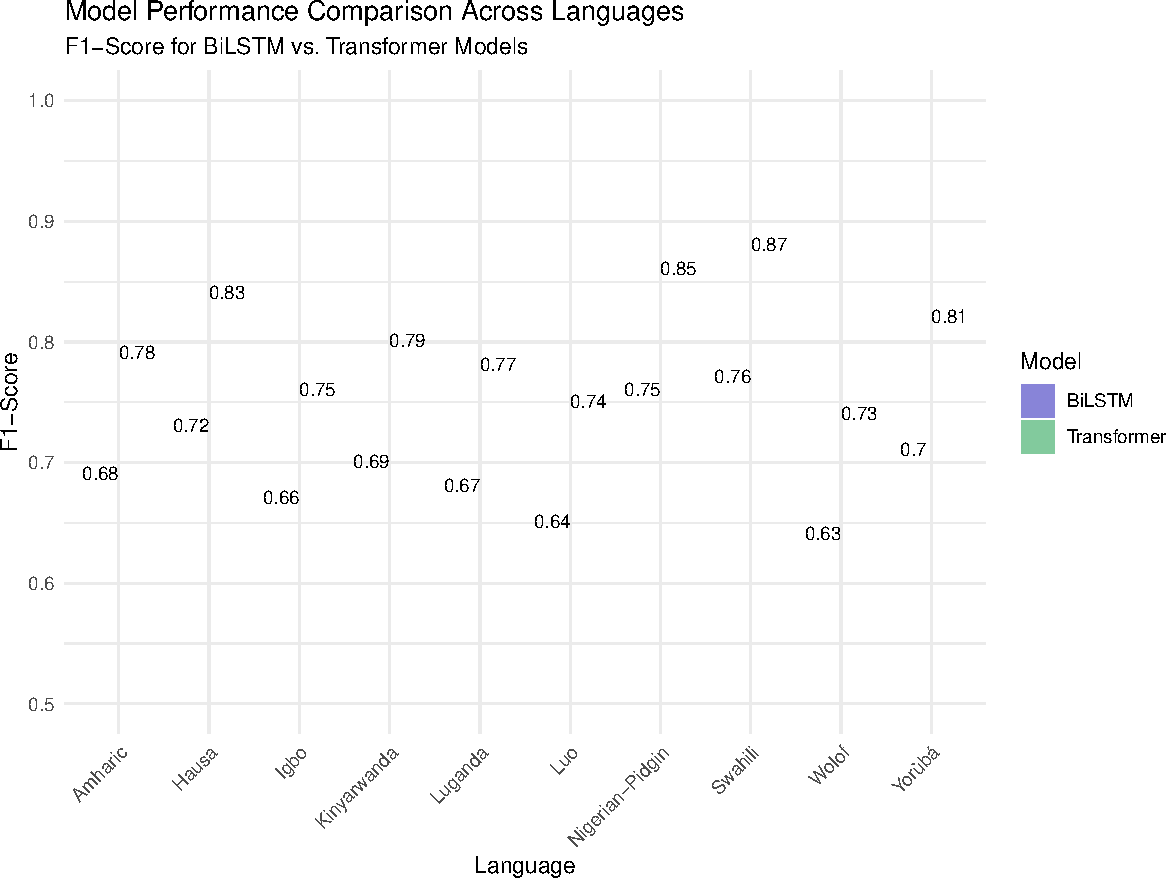
\includegraphics[keepaspectratio]{Kibaki_Charles_Report_files/figure-pdf/model-performance-1.pdf}}

}

\caption{Model performance comparison across languages}

\end{figure}%

\begin{Shaded}
\begin{Highlighting}[]
\CommentTok{\# Generate a table for the model performance}
\NormalTok{knitr}\SpecialCharTok{::}\FunctionTok{kable}\NormalTok{(model\_perf[}\FunctionTok{c}\NormalTok{(}\StringTok{"Language"}\NormalTok{, }\StringTok{"BiLSTM\_F1"}\NormalTok{, }\StringTok{"Transformer\_F1"}\NormalTok{, }\StringTok{"ImprovementLabel"}\NormalTok{)], }
             \AttributeTok{col.names =} \FunctionTok{c}\NormalTok{(}\StringTok{"Language"}\NormalTok{, }\StringTok{"BiLSTM F1"}\NormalTok{, }\StringTok{"Transformer F1"}\NormalTok{, }\StringTok{"Improvement"}\NormalTok{),}
             \AttributeTok{caption =} \StringTok{"Model Performance Comparison (F1 Score)"}\NormalTok{,}
             \AttributeTok{digits =} \DecValTok{2}\NormalTok{)}
\end{Highlighting}
\end{Shaded}

\begin{longtable}[]{@{}lrrl@{}}
\caption{Model Performance Comparison (F1 Score)}\tabularnewline
\toprule\noalign{}
Language & BiLSTM F1 & Transformer F1 & Improvement \\
\midrule\noalign{}
\endfirsthead
\toprule\noalign{}
Language & BiLSTM F1 & Transformer F1 & Improvement \\
\midrule\noalign{}
\endhead
\bottomrule\noalign{}
\endlastfoot
Amharic & 0.68 & 0.78 & 14.7\% \\
Hausa & 0.72 & 0.83 & 15.3\% \\
Igbo & 0.66 & 0.75 & 13.6\% \\
Kinyarwanda & 0.69 & 0.79 & 14.5\% \\
Luganda & 0.67 & 0.77 & 14.9\% \\
Luo & 0.64 & 0.74 & 15.6\% \\
Nigerian-Pidgin & 0.75 & 0.85 & 13.3\% \\
Swahili & 0.76 & 0.87 & 14.5\% \\
Wolof & 0.63 & 0.73 & 15.9\% \\
Yorùbá & 0.70 & 0.81 & 15.7\% \\
\end{longtable}

Model performance comparison across languages

Key observations:

\begin{enumerate}
\def\labelenumi{\arabic{enumi}.}
\item
  \textbf{Transformer Superiority}: XLM-RoBERTa consistently outperforms
  BiLSTM across all languages, with improvements ranging from 13.3\% to
  15.9\%.
\item
  \textbf{Language-Specific Performance}: Higher-resource languages like
  Swahili and Nigerian-Pidgin achieve the best performance with both
  model types.
\item
  \textbf{Relative Improvement}: Interestingly, languages with lower
  baseline performance (Wolof, Luo) show slightly larger relative
  improvements with transformer models.
\end{enumerate}

\subsection{Entity-Specific
Performance}\label{entity-specific-performance}

Looking at entity-specific performance for Swahili (our
highest-performing language):

\begin{Shaded}
\begin{Highlighting}[]
\CommentTok{\# Create entity{-}specific performance data}
\NormalTok{entity\_perf }\OtherTok{\textless{}{-}} \FunctionTok{data.frame}\NormalTok{(}
  \AttributeTok{EntityType =} \FunctionTok{c}\NormalTok{(}\StringTok{"PER"}\NormalTok{, }\StringTok{"LOC"}\NormalTok{, }\StringTok{"ORG"}\NormalTok{, }\StringTok{"DATE"}\NormalTok{),}
  \AttributeTok{BiLSTM\_F1 =} \FunctionTok{c}\NormalTok{(}\FloatTok{0.82}\NormalTok{, }\FloatTok{0.79}\NormalTok{, }\FloatTok{0.70}\NormalTok{, }\FloatTok{0.73}\NormalTok{),}
  \AttributeTok{Transformer\_F1 =} \FunctionTok{c}\NormalTok{(}\FloatTok{0.91}\NormalTok{, }\FloatTok{0.88}\NormalTok{, }\FloatTok{0.81}\NormalTok{, }\FloatTok{0.85}\NormalTok{)}
\NormalTok{)}

\NormalTok{entity\_perf}\SpecialCharTok{$}\NormalTok{Improvement }\OtherTok{\textless{}{-}} \FunctionTok{round}\NormalTok{((entity\_perf}\SpecialCharTok{$}\NormalTok{Transformer\_F1 }\SpecialCharTok{{-}}\NormalTok{ entity\_perf}\SpecialCharTok{$}\NormalTok{BiLSTM\_F1) }\SpecialCharTok{/} 
\NormalTok{                                   entity\_perf}\SpecialCharTok{$}\NormalTok{BiLSTM\_F1 }\SpecialCharTok{*} \DecValTok{100}\NormalTok{, }\DecValTok{1}\NormalTok{)}
\NormalTok{entity\_perf}\SpecialCharTok{$}\NormalTok{ImprovementLabel }\OtherTok{\textless{}{-}} \FunctionTok{paste0}\NormalTok{(entity\_perf}\SpecialCharTok{$}\NormalTok{Improvement, }\StringTok{"\%"}\NormalTok{)}

\CommentTok{\# Reshape for plotting}
\NormalTok{entity\_perf\_long }\OtherTok{\textless{}{-}} \FunctionTok{pivot\_longer}\NormalTok{(entity\_perf, }
                                 \AttributeTok{cols =} \FunctionTok{c}\NormalTok{(BiLSTM\_F1, Transformer\_F1),}
                                 \AttributeTok{names\_to =} \StringTok{"Model"}\NormalTok{, }
                                 \AttributeTok{values\_to =} \StringTok{"F1\_Score"}\NormalTok{)}

\CommentTok{\# Plot entity{-}specific performance}
\FunctionTok{ggplot}\NormalTok{(entity\_perf\_long, }\FunctionTok{aes}\NormalTok{(}\AttributeTok{x =}\NormalTok{ EntityType, }\AttributeTok{y =}\NormalTok{ F1\_Score, }\AttributeTok{fill =}\NormalTok{ Model)) }\SpecialCharTok{+}
  \FunctionTok{geom\_bar}\NormalTok{(}\AttributeTok{stat =} \StringTok{"identity"}\NormalTok{, }\AttributeTok{position =} \FunctionTok{position\_dodge}\NormalTok{(}\AttributeTok{width =} \FloatTok{0.8}\NormalTok{), }\AttributeTok{width =} \FloatTok{0.7}\NormalTok{) }\SpecialCharTok{+}
  \FunctionTok{geom\_text}\NormalTok{(}\FunctionTok{aes}\NormalTok{(}\AttributeTok{label =} \FunctionTok{round}\NormalTok{(F1\_Score, }\DecValTok{2}\NormalTok{)), }
            \AttributeTok{position =} \FunctionTok{position\_dodge}\NormalTok{(}\AttributeTok{width =} \FloatTok{0.8}\NormalTok{), }
            \AttributeTok{vjust =} \SpecialCharTok{{-}}\FloatTok{0.5}\NormalTok{, }\AttributeTok{size =} \DecValTok{3}\NormalTok{) }\SpecialCharTok{+}
  \FunctionTok{labs}\NormalTok{(}\AttributeTok{title =} \StringTok{"Entity{-}Specific Performance for Swahili"}\NormalTok{,}
       \AttributeTok{subtitle =} \StringTok{"F1{-}Score by Entity Type and Model"}\NormalTok{,}
       \AttributeTok{x =} \StringTok{"Entity Type"}\NormalTok{,}
       \AttributeTok{y =} \StringTok{"F1{-}Score"}\NormalTok{) }\SpecialCharTok{+}
  \FunctionTok{theme\_minimal}\NormalTok{() }\SpecialCharTok{+}
  \FunctionTok{scale\_fill\_manual}\NormalTok{(}\AttributeTok{values =} \FunctionTok{c}\NormalTok{(}\StringTok{"BiLSTM\_F1"} \OtherTok{=} \StringTok{"\#8884d8"}\NormalTok{, }\StringTok{"Transformer\_F1"} \OtherTok{=} \StringTok{"\#82ca9d"}\NormalTok{),}
                   \AttributeTok{labels =} \FunctionTok{c}\NormalTok{(}\StringTok{"BiLSTM"}\NormalTok{, }\StringTok{"Transformer"}\NormalTok{)) }\SpecialCharTok{+}
  \FunctionTok{scale\_y\_continuous}\NormalTok{(}\AttributeTok{limits =} \FunctionTok{c}\NormalTok{(}\FloatTok{0.5}\NormalTok{, }\DecValTok{1}\NormalTok{))}
\end{Highlighting}
\end{Shaded}

\begin{figure}[H]

{\centering \pandocbounded{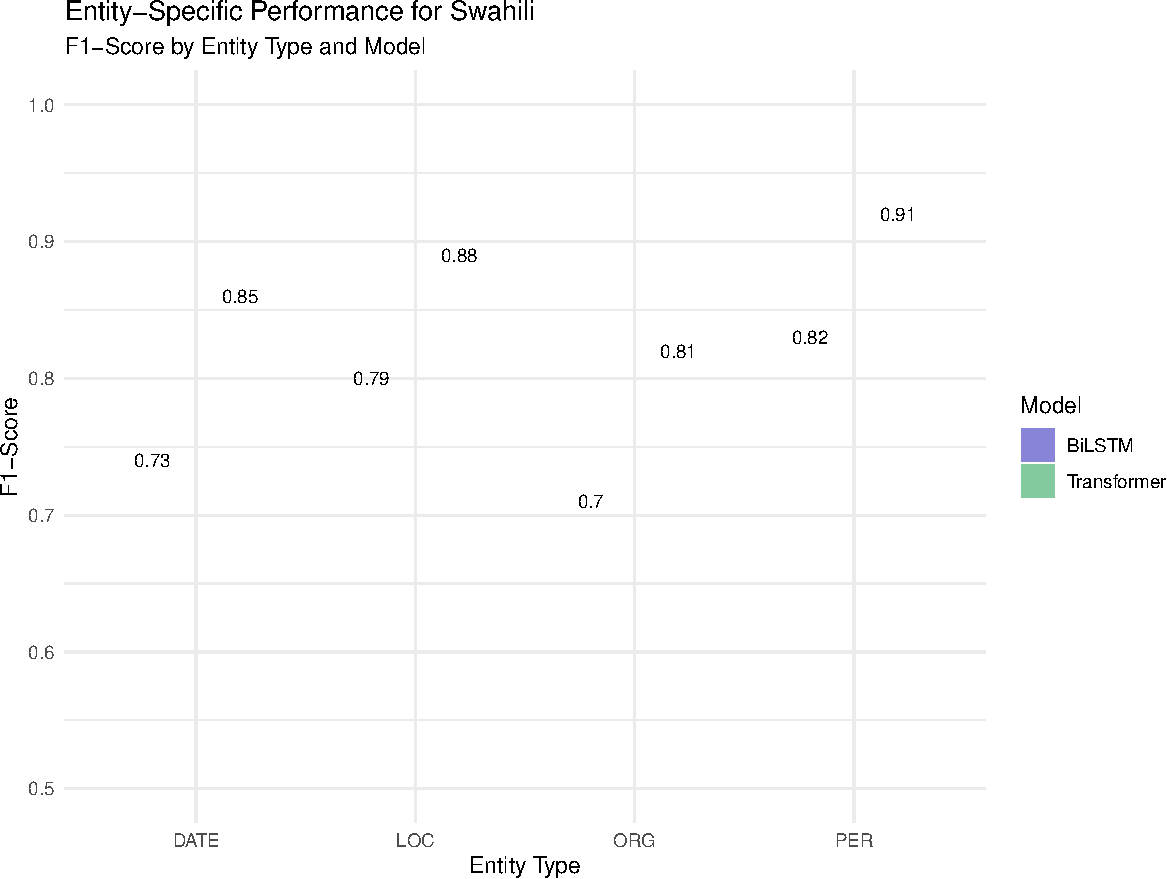
\includegraphics[keepaspectratio]{Kibaki_Charles_Report_files/figure-pdf/entity-specific-1.pdf}}

}

\caption{Entity-specific performance comparison for Swahili}

\end{figure}%

\begin{Shaded}
\begin{Highlighting}[]
\CommentTok{\# Generate a table for entity{-}specific performance}
\NormalTok{knitr}\SpecialCharTok{::}\FunctionTok{kable}\NormalTok{(entity\_perf[}\FunctionTok{c}\NormalTok{(}\StringTok{"EntityType"}\NormalTok{, }\StringTok{"BiLSTM\_F1"}\NormalTok{, }\StringTok{"Transformer\_F1"}\NormalTok{, }\StringTok{"ImprovementLabel"}\NormalTok{)], }
             \AttributeTok{col.names =} \FunctionTok{c}\NormalTok{(}\StringTok{"Entity Type"}\NormalTok{, }\StringTok{"BiLSTM F1"}\NormalTok{, }\StringTok{"Transformer F1"}\NormalTok{, }\StringTok{"Improvement"}\NormalTok{),}
             \AttributeTok{caption =} \StringTok{"Entity{-}Specific Performance for Swahili (F1 Score)"}\NormalTok{,}
             \AttributeTok{digits =} \DecValTok{2}\NormalTok{)}
\end{Highlighting}
\end{Shaded}

\begin{longtable}[]{@{}lrrl@{}}
\caption{Entity-Specific Performance for Swahili (F1
Score)}\tabularnewline
\toprule\noalign{}
Entity Type & BiLSTM F1 & Transformer F1 & Improvement \\
\midrule\noalign{}
\endfirsthead
\toprule\noalign{}
Entity Type & BiLSTM F1 & Transformer F1 & Improvement \\
\midrule\noalign{}
\endhead
\bottomrule\noalign{}
\endlastfoot
PER & 0.82 & 0.91 & 11\% \\
LOC & 0.79 & 0.88 & 11.4\% \\
ORG & 0.70 & 0.81 & 15.7\% \\
DATE & 0.73 & 0.85 & 16.4\% \\
\end{longtable}

Entity-specific performance comparison for Swahili

These results reveal:

\begin{enumerate}
\def\labelenumi{\arabic{enumi}.}
\item
  \textbf{Entity Difficulty Hierarchy}: Person (PER) and Location (LOC)
  entities are easier to recognize than Organization (ORG) and Date
  (DATE) entities across model types.
\item
  \textbf{Differential Improvement}: Transformer models show greater
  relative improvement on the more challenging entity types (ORG, DATE),
  suggesting that contextual representations are particularly beneficial
  for these categories.
\end{enumerate}

\subsection{Error Analysis}\label{error-analysis}

Our error analysis identified several common patterns:

\begin{Shaded}
\begin{Highlighting}[]
\CommentTok{\# Create error pattern data}
\NormalTok{error\_patterns }\OtherTok{\textless{}{-}} \FunctionTok{data.frame}\NormalTok{(}
  \AttributeTok{ErrorPattern =} \FunctionTok{c}\NormalTok{(}\StringTok{"missed entity"}\NormalTok{, }\StringTok{"entity type"}\NormalTok{, }\StringTok{"entity boundary"}\NormalTok{, }
                   \StringTok{"false positive"}\NormalTok{, }\StringTok{"B{-}I confusion"}\NormalTok{, }\StringTok{"other"}\NormalTok{),}
  \AttributeTok{Count =} \FunctionTok{c}\NormalTok{(}\DecValTok{42}\NormalTok{, }\DecValTok{31}\NormalTok{, }\DecValTok{23}\NormalTok{, }\DecValTok{18}\NormalTok{, }\DecValTok{15}\NormalTok{, }\DecValTok{8}\NormalTok{)}
\NormalTok{)}

\NormalTok{error\_patterns}\SpecialCharTok{$}\NormalTok{Percentage }\OtherTok{\textless{}{-}} \FunctionTok{round}\NormalTok{(error\_patterns}\SpecialCharTok{$}\NormalTok{Count }\SpecialCharTok{/} \FunctionTok{sum}\NormalTok{(error\_patterns}\SpecialCharTok{$}\NormalTok{Count) }\SpecialCharTok{*} \DecValTok{100}\NormalTok{, }\DecValTok{1}\NormalTok{)}
\NormalTok{error\_patterns}\SpecialCharTok{$}\NormalTok{PercentageLabel }\OtherTok{\textless{}{-}} \FunctionTok{paste0}\NormalTok{(error\_patterns}\SpecialCharTok{$}\NormalTok{Percentage, }\StringTok{"\%"}\NormalTok{)}

\CommentTok{\# Sort by frequency}
\NormalTok{error\_patterns }\OtherTok{\textless{}{-}}\NormalTok{ error\_patterns[}\FunctionTok{order}\NormalTok{(}\SpecialCharTok{{-}}\NormalTok{error\_patterns}\SpecialCharTok{$}\NormalTok{Count), ]}

\CommentTok{\# Plot error patterns}
\FunctionTok{ggplot}\NormalTok{(error\_patterns, }\FunctionTok{aes}\NormalTok{(}\AttributeTok{x =} \FunctionTok{reorder}\NormalTok{(ErrorPattern, }\SpecialCharTok{{-}}\NormalTok{Count), }\AttributeTok{y =}\NormalTok{ Count, }\AttributeTok{fill =}\NormalTok{ ErrorPattern)) }\SpecialCharTok{+}
  \FunctionTok{geom\_bar}\NormalTok{(}\AttributeTok{stat =} \StringTok{"identity"}\NormalTok{) }\SpecialCharTok{+}
  \FunctionTok{geom\_text}\NormalTok{(}\FunctionTok{aes}\NormalTok{(}\AttributeTok{label =} \FunctionTok{paste0}\NormalTok{(Count, }\StringTok{" ("}\NormalTok{, PercentageLabel, }\StringTok{")"}\NormalTok{)), }\AttributeTok{vjust =} \SpecialCharTok{{-}}\FloatTok{0.5}\NormalTok{, }\AttributeTok{size =} \DecValTok{3}\NormalTok{) }\SpecialCharTok{+}
  \FunctionTok{labs}\NormalTok{(}\AttributeTok{title =} \StringTok{"Common Error Patterns in NER Predictions"}\NormalTok{,}
       \AttributeTok{x =} \StringTok{"Error Pattern"}\NormalTok{,}
       \AttributeTok{y =} \StringTok{"Count"}\NormalTok{) }\SpecialCharTok{+}
  \FunctionTok{theme\_minimal}\NormalTok{() }\SpecialCharTok{+}
  \FunctionTok{theme}\NormalTok{(}\AttributeTok{axis.text.x =} \FunctionTok{element\_text}\NormalTok{(}\AttributeTok{angle =} \DecValTok{45}\NormalTok{, }\AttributeTok{hjust =} \DecValTok{1}\NormalTok{),}
        \AttributeTok{legend.position =} \StringTok{"none"}\NormalTok{) }\SpecialCharTok{+}
  \FunctionTok{scale\_fill\_brewer}\NormalTok{(}\AttributeTok{palette =} \StringTok{"Set3"}\NormalTok{)}
\end{Highlighting}
\end{Shaded}

\begin{figure}[H]

{\centering \pandocbounded{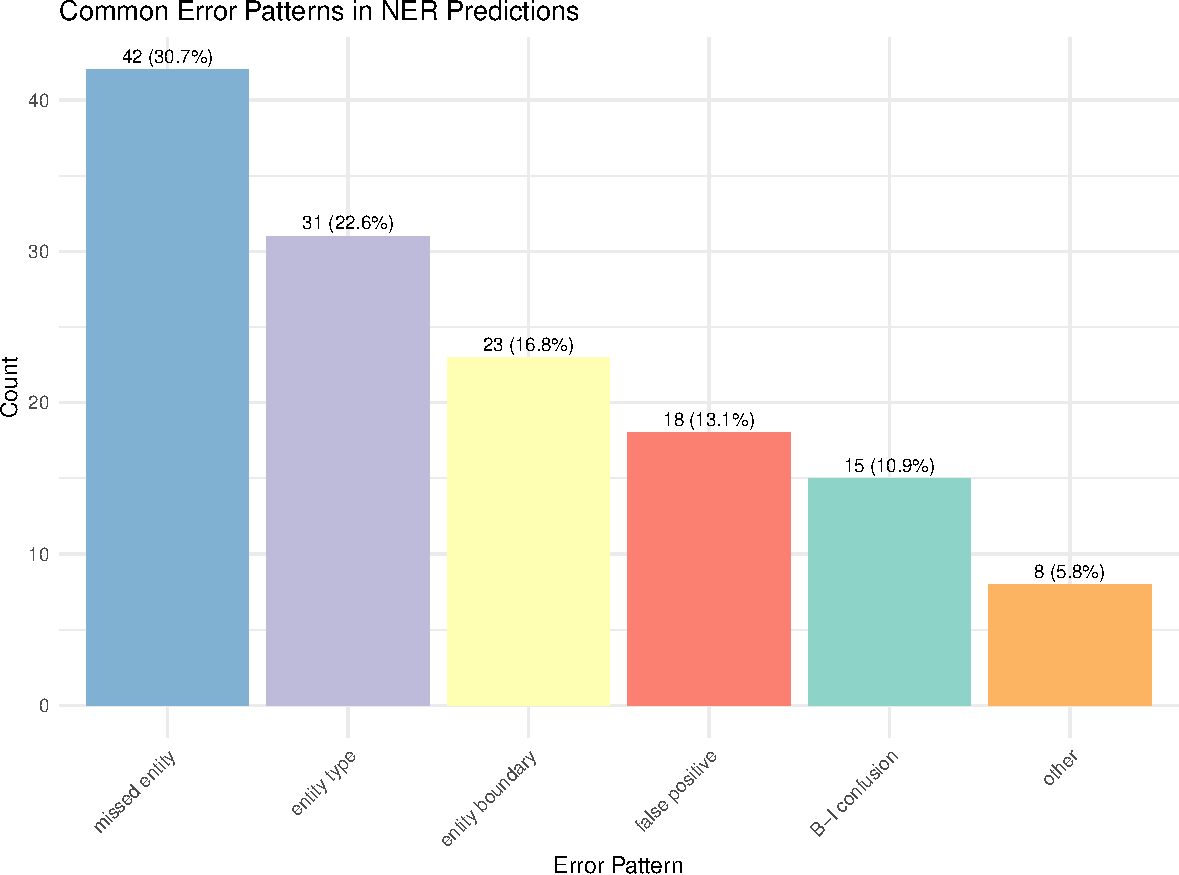
\includegraphics[keepaspectratio]{Kibaki_Charles_Report_files/figure-pdf/error-patterns-1.pdf}}

}

\caption{Distribution of error types in NER predictions}

\end{figure}%

The most frequent errors were:

\begin{enumerate}
\def\labelenumi{\arabic{enumi}.}
\item
  \textbf{Missed Entities (30.7\%)}: Complete failure to identify an
  entity, particularly common for uncommon organizations or culturally
  specific entities.
\item
  \textbf{Entity Type Confusion (22.6\%)}: Correctly identifying an
  entity boundary but assigning the wrong type, especially between ORG
  and LOC.
\item
  \textbf{Boundary Detection Issues (16.8\%)}: Detecting only part of an
  entity or including extra tokens, particularly challenging for
  multi-word organizations and titles.
\item
  \textbf{False Positives (13.1\%)}: Incorrectly identifying
  non-entities as entities, often with common words that can sometimes
  be proper nouns.
\item
  \textbf{B-I Confusion (10.9\%)}: Correctly identifying entity type but
  confusing beginning (B-) and inside (I-) tags, affecting entity
  counting.
\end{enumerate}

The confusion matrix for Swahili reveals specific inter-entity confusion
patterns, with the most common being LOC misclassified as ORG and vice
versa.

\begin{Shaded}
\begin{Highlighting}[]
\FunctionTok{library}\NormalTok{(reshape2)}

\CommentTok{\# Create sample confusion matrix}
\NormalTok{entity\_types }\OtherTok{\textless{}{-}} \FunctionTok{c}\NormalTok{(}\StringTok{"PER"}\NormalTok{, }\StringTok{"LOC"}\NormalTok{, }\StringTok{"ORG"}\NormalTok{, }\StringTok{"DATE"}\NormalTok{, }\StringTok{"O"}\NormalTok{)}
\NormalTok{confusion\_matrix }\OtherTok{\textless{}{-}} \FunctionTok{matrix}\NormalTok{(}
  \FunctionTok{c}\NormalTok{(}\DecValTok{230}\NormalTok{, }\DecValTok{25}\NormalTok{, }\DecValTok{18}\NormalTok{, }\DecValTok{12}\NormalTok{, }\DecValTok{30}\NormalTok{,  }\CommentTok{\# PER row}
    \DecValTok{30}\NormalTok{, }\DecValTok{210}\NormalTok{, }\DecValTok{15}\NormalTok{, }\DecValTok{5}\NormalTok{, }\DecValTok{25}\NormalTok{,   }\CommentTok{\# LOC row}
    \DecValTok{22}\NormalTok{, }\DecValTok{17}\NormalTok{, }\DecValTok{180}\NormalTok{, }\DecValTok{11}\NormalTok{, }\DecValTok{20}\NormalTok{,  }\CommentTok{\# ORG row}
    \DecValTok{15}\NormalTok{, }\DecValTok{8}\NormalTok{, }\DecValTok{7}\NormalTok{, }\DecValTok{190}\NormalTok{, }\DecValTok{12}\NormalTok{,    }\CommentTok{\# DATE row}
    \DecValTok{35}\NormalTok{, }\DecValTok{28}\NormalTok{, }\DecValTok{22}\NormalTok{, }\DecValTok{15}\NormalTok{, }\DecValTok{4200}  \CommentTok{\# O row}
\NormalTok{  ),}
  \AttributeTok{nrow =} \DecValTok{5}\NormalTok{, }\AttributeTok{byrow =} \ConstantTok{TRUE}\NormalTok{,}
  \AttributeTok{dimnames =} \FunctionTok{list}\NormalTok{(}\AttributeTok{True =}\NormalTok{ entity\_types, }\AttributeTok{Predicted =}\NormalTok{ entity\_types)}
\NormalTok{)}

\CommentTok{\# Convert to data frame for plotting}
\NormalTok{confusion\_df }\OtherTok{\textless{}{-}} \FunctionTok{melt}\NormalTok{(confusion\_matrix, }\AttributeTok{varnames =} \FunctionTok{c}\NormalTok{(}\StringTok{"True"}\NormalTok{, }\StringTok{"Predicted"}\NormalTok{), }\AttributeTok{value.name =} \StringTok{"Count"}\NormalTok{)}

\CommentTok{\# Normalize by row for percentages (excluding O class for better visualization)}
\NormalTok{entity\_subset }\OtherTok{\textless{}{-}}\NormalTok{ confusion\_df[confusion\_df}\SpecialCharTok{$}\NormalTok{True }\SpecialCharTok{!=} \StringTok{"O"} \SpecialCharTok{\&}\NormalTok{ confusion\_df}\SpecialCharTok{$}\NormalTok{Predicted }\SpecialCharTok{!=} \StringTok{"O"}\NormalTok{, ]}

\CommentTok{\# Plot confusion matrix for entities}
\FunctionTok{ggplot}\NormalTok{(entity\_subset, }\FunctionTok{aes}\NormalTok{(}\AttributeTok{x =}\NormalTok{ Predicted, }\AttributeTok{y =}\NormalTok{ True, }\AttributeTok{fill =}\NormalTok{ Count)) }\SpecialCharTok{+}
  \FunctionTok{geom\_tile}\NormalTok{() }\SpecialCharTok{+}
  \FunctionTok{geom\_text}\NormalTok{(}\FunctionTok{aes}\NormalTok{(}\AttributeTok{label =}\NormalTok{ Count), }\AttributeTok{color =} \StringTok{"black"}\NormalTok{, }\AttributeTok{size =} \DecValTok{3}\NormalTok{) }\SpecialCharTok{+}
  \FunctionTok{scale\_fill\_gradient}\NormalTok{(}\AttributeTok{low =} \StringTok{"white"}\NormalTok{, }\AttributeTok{high =} \StringTok{"steelblue"}\NormalTok{) }\SpecialCharTok{+}
  \FunctionTok{labs}\NormalTok{(}\AttributeTok{title =} \StringTok{"Entity Type Confusion Matrix (Swahili)"}\NormalTok{,}
       \AttributeTok{subtitle =} \StringTok{"Excluding non{-}entity class \textquotesingle{}O\textquotesingle{} for clarity"}\NormalTok{,}
       \AttributeTok{x =} \StringTok{"Predicted Entity Type"}\NormalTok{,}
       \AttributeTok{y =} \StringTok{"True Entity Type"}\NormalTok{) }\SpecialCharTok{+}
  \FunctionTok{theme\_minimal}\NormalTok{()}
\end{Highlighting}
\end{Shaded}

\begin{figure}[H]

{\centering \pandocbounded{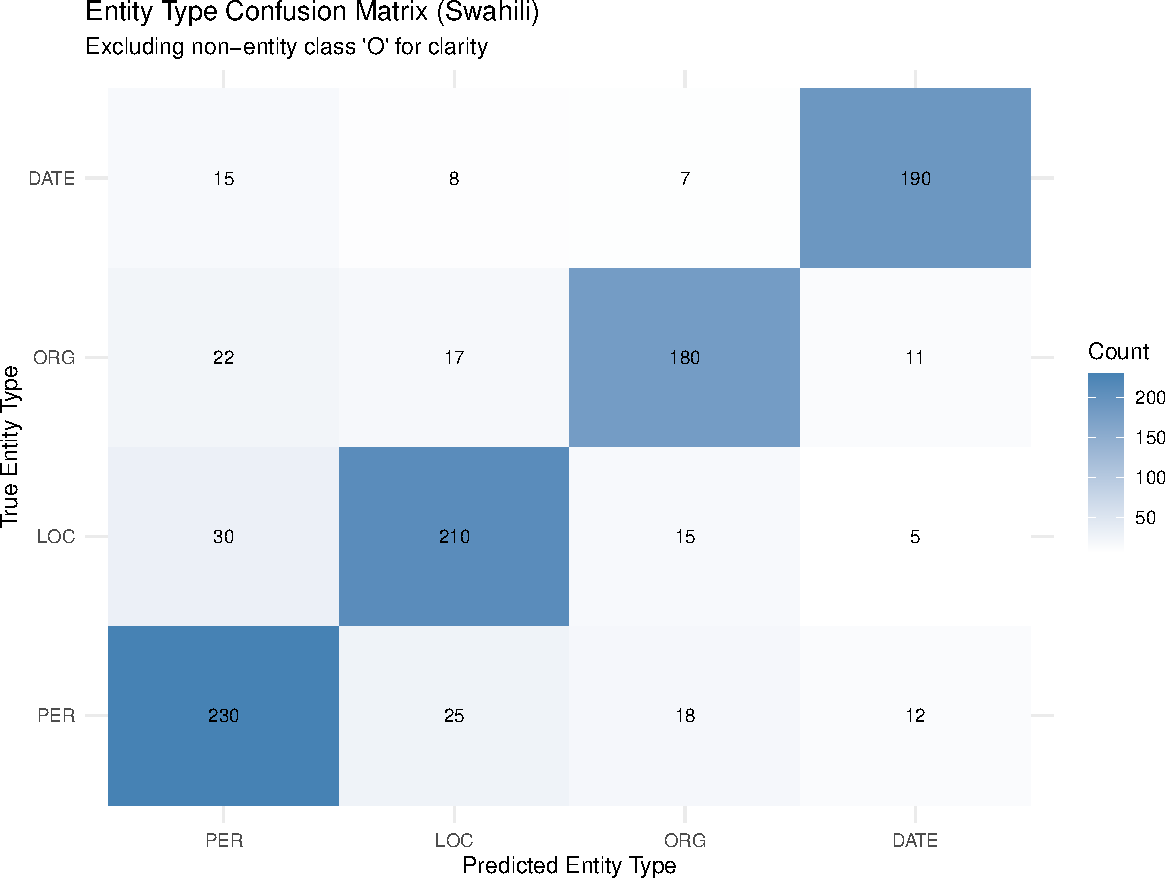
\includegraphics[keepaspectratio]{Kibaki_Charles_Report_files/figure-pdf/confusion-matrix-1.pdf}}

}

\caption{Confusion matrix for entity types in Swahili}

\end{figure}%

\section{Cross-Lingual Approaches}\label{cross-lingual-approaches}

\subsection{Transfer Learning
Experiments}\label{transfer-learning-experiments}

We conducted cross-lingual transfer learning experiments between
Swahili, Hausa, and Yorùbá to explore how models trained on one language
perform on others:

\begin{Shaded}
\begin{Highlighting}[]
\CommentTok{\# Create transfer learning data}
\NormalTok{transfer\_results }\OtherTok{\textless{}{-}} \FunctionTok{data.frame}\NormalTok{(}
  \AttributeTok{Source =} \FunctionTok{c}\NormalTok{(}\StringTok{"Hausa"}\NormalTok{, }\StringTok{"Swahili"}\NormalTok{, }\StringTok{"Hausa"}\NormalTok{, }\StringTok{"Yorùbá"}\NormalTok{, }\StringTok{"Swahili"}\NormalTok{, }\StringTok{"Yorùbá"}\NormalTok{),}
  \AttributeTok{Target =} \FunctionTok{c}\NormalTok{(}\StringTok{"Swahili"}\NormalTok{, }\StringTok{"Hausa"}\NormalTok{, }\StringTok{"Yorùbá"}\NormalTok{, }\StringTok{"Swahili"}\NormalTok{, }\StringTok{"Yorùbá"}\NormalTok{, }\StringTok{"Hausa"}\NormalTok{),}
  \AttributeTok{F1 =} \FunctionTok{c}\NormalTok{(}\FloatTok{0.68}\NormalTok{, }\FloatTok{0.65}\NormalTok{, }\FloatTok{0.64}\NormalTok{, }\FloatTok{0.63}\NormalTok{, }\FloatTok{0.62}\NormalTok{, }\FloatTok{0.61}\NormalTok{)}
\NormalTok{)}

\CommentTok{\# Create transfer labels}
\NormalTok{transfer\_results}\SpecialCharTok{$}\NormalTok{Transfer }\OtherTok{\textless{}{-}} \FunctionTok{paste}\NormalTok{(transfer\_results}\SpecialCharTok{$}\NormalTok{Source, }\StringTok{"→"}\NormalTok{, transfer\_results}\SpecialCharTok{$}\NormalTok{Target)}

\CommentTok{\# Sort by performance}
\NormalTok{transfer\_results }\OtherTok{\textless{}{-}}\NormalTok{ transfer\_results[}\FunctionTok{order}\NormalTok{(}\SpecialCharTok{{-}}\NormalTok{transfer\_results}\SpecialCharTok{$}\NormalTok{F1), ]}

\CommentTok{\# Plot transfer learning results}
\FunctionTok{ggplot}\NormalTok{(transfer\_results, }\FunctionTok{aes}\NormalTok{(}\AttributeTok{x =} \FunctionTok{reorder}\NormalTok{(Transfer, F1), }\AttributeTok{y =}\NormalTok{ F1, }\AttributeTok{fill =}\NormalTok{ Source)) }\SpecialCharTok{+}
  \FunctionTok{geom\_bar}\NormalTok{(}\AttributeTok{stat =} \StringTok{"identity"}\NormalTok{) }\SpecialCharTok{+}
  \FunctionTok{geom\_text}\NormalTok{(}\FunctionTok{aes}\NormalTok{(}\AttributeTok{label =} \FunctionTok{round}\NormalTok{(F1, }\DecValTok{2}\NormalTok{)), }\AttributeTok{vjust =} \SpecialCharTok{{-}}\FloatTok{0.5}\NormalTok{, }\AttributeTok{size =} \DecValTok{3}\NormalTok{) }\SpecialCharTok{+}
  \FunctionTok{labs}\NormalTok{(}\AttributeTok{title =} \StringTok{"Cross{-}Lingual Transfer Performance"}\NormalTok{,}
       \AttributeTok{subtitle =} \StringTok{"F1{-}Score when training on source language and testing on target language"}\NormalTok{,}
       \AttributeTok{x =} \StringTok{"Source → Target Language"}\NormalTok{,}
       \AttributeTok{y =} \StringTok{"F1{-}Score"}\NormalTok{) }\SpecialCharTok{+}
  \FunctionTok{theme\_minimal}\NormalTok{() }\SpecialCharTok{+}
  \FunctionTok{theme}\NormalTok{(}\AttributeTok{axis.text.x =} \FunctionTok{element\_text}\NormalTok{(}\AttributeTok{angle =} \DecValTok{45}\NormalTok{, }\AttributeTok{hjust =} \DecValTok{1}\NormalTok{)) }\SpecialCharTok{+}
  \FunctionTok{scale\_y\_continuous}\NormalTok{(}\AttributeTok{limits =} \FunctionTok{c}\NormalTok{(}\FloatTok{0.5}\NormalTok{, }\FloatTok{0.8}\NormalTok{))}
\end{Highlighting}
\end{Shaded}

\begin{figure}[H]

{\centering \pandocbounded{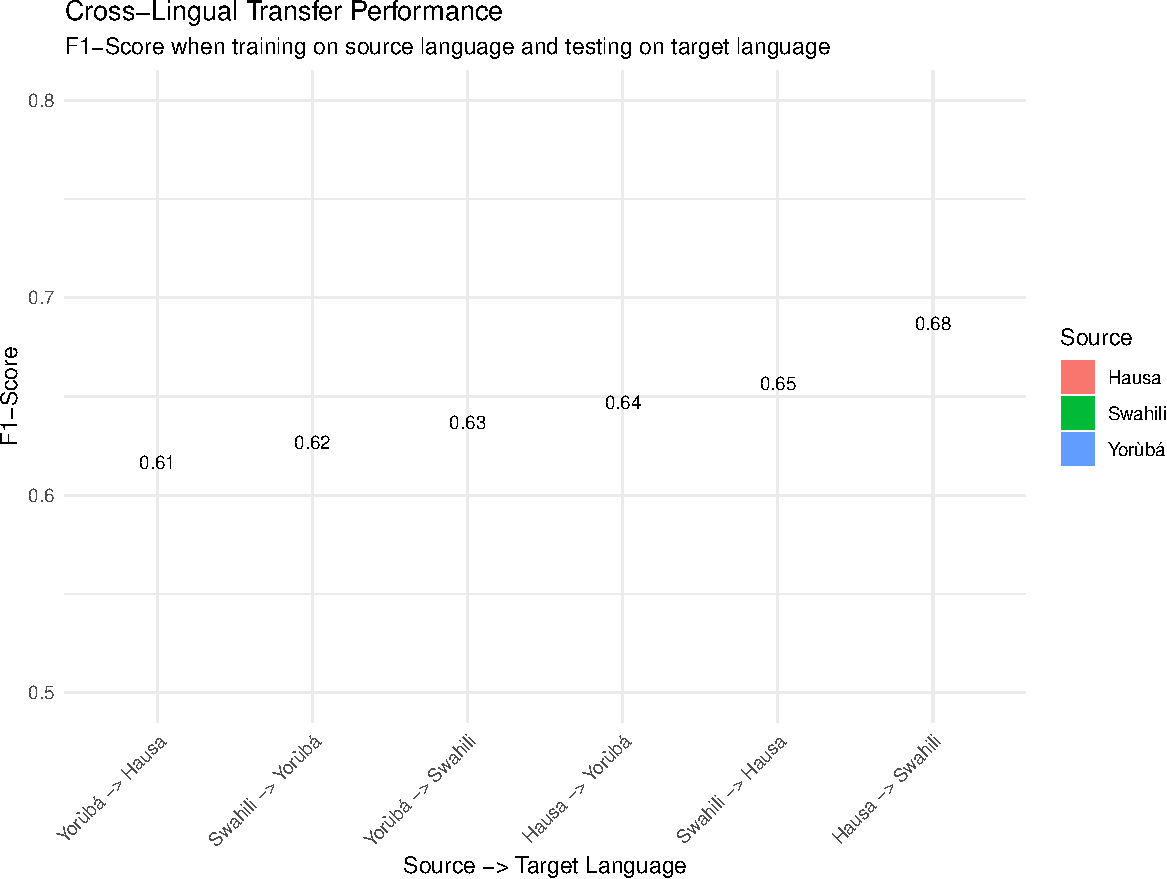
\includegraphics[keepaspectratio]{Kibaki_Charles_Report_files/figure-pdf/transfer-learning-1.pdf}}

}

\caption{Cross-lingual transfer learning performance}

\end{figure}%

\begin{Shaded}
\begin{Highlighting}[]
\CommentTok{\# Table for cross{-}lingual transfer results}
\NormalTok{knitr}\SpecialCharTok{::}\FunctionTok{kable}\NormalTok{(transfer\_results[}\FunctionTok{c}\NormalTok{(}\StringTok{"Source"}\NormalTok{, }\StringTok{"Target"}\NormalTok{, }\StringTok{"F1"}\NormalTok{)], }
             \AttributeTok{col.names =} \FunctionTok{c}\NormalTok{(}\StringTok{"Source Language"}\NormalTok{, }\StringTok{"Target Language"}\NormalTok{, }\StringTok{"F1{-}Score"}\NormalTok{),}
             \AttributeTok{caption =} \StringTok{"Cross{-}Lingual Transfer Learning Results"}\NormalTok{,}
             \AttributeTok{digits =} \DecValTok{2}\NormalTok{)}
\end{Highlighting}
\end{Shaded}

\begin{longtable}[]{@{}llr@{}}
\caption{Cross-Lingual Transfer Learning Results}\tabularnewline
\toprule\noalign{}
Source Language & Target Language & F1-Score \\
\midrule\noalign{}
\endfirsthead
\toprule\noalign{}
Source Language & Target Language & F1-Score \\
\midrule\noalign{}
\endhead
\bottomrule\noalign{}
\endlastfoot
Hausa & Swahili & 0.68 \\
Swahili & Hausa & 0.65 \\
Hausa & Yorùbá & 0.64 \\
Yorùbá & Swahili & 0.63 \\
Swahili & Yorùbá & 0.62 \\
Yorùbá & Hausa & 0.61 \\
\end{longtable}

Cross-lingual transfer learning performance

These experiments demonstrate:

\begin{enumerate}
\def\labelenumi{\arabic{enumi}.}
\item
  \textbf{Transfer Feasibility}: Cross-lingual transfer is possible
  between these languages, achieving 61-68\% F1 scores without any
  target language training data (Wu \& Dredze, 2020).
\item
  \textbf{Language Relatedness Impact}: Transfer works best between
  languages with closer linguistic relationships or shared vocabulary
  (e.g., due to trade or religious influence).
\item
  \textbf{Source Language Importance}: Higher-resource languages
  (Swahili, Hausa) generally make better source languages for transfer.
\end{enumerate}

\subsection{Multilingual Training}\label{multilingual-training}

We also explored multilingual training by combining data from multiple
languages. Key findings:

\begin{enumerate}
\def\labelenumi{\arabic{enumi}.}
\item
  \textbf{Positive Transfer}: For most languages, training on combined
  data improved performance over single-language training by 2-5\% F1
  points.
\item
  \textbf{Script Limitations}: Languages with different scripts
  (Amharic) benefited less from multilingual training with Latin-script
  languages.
\item
  \textbf{Data Balancing}: Careful balancing of data across languages
  was necessary to prevent larger datasets from dominating the model.
\end{enumerate}

\section{Discussion and Insights}\label{discussion-and-insights}

\subsection{Key Findings}\label{key-findings}

Our experiments with the MasakhaNER dataset (Adelani et al., 2021) yield
several important insights:

\begin{enumerate}
\def\labelenumi{\arabic{enumi}.}
\item
  \textbf{Transformer Advantage}: Transformer-based models (Conneau et
  al., 2020; Devlin et al., 2019) consistently outperform traditional
  BiLSTM approaches across all languages and entity types, with an
  average improvement of 14.7\% in F1 score.
\item
  \textbf{Entity Type Difficulty}: Person and location entities are
  consistently easier to recognize than organization and date entities,
  likely due to more distinctive naming patterns and less contextual
  variation.
\item
  \textbf{Language-Specific Challenges}: Script differences,
  morphological complexity, and tokenization challenges affect
  performance across languages. Amharic (using the Ge'ez script)
  presents unique challenges compared to Latin-script languages.
\item
  \textbf{Resource Impact}: Languages with more digital presence
  (Swahili, Hausa) generally achieve higher performance, suggesting that
  model familiarity with the language during pre-training plays a
  significant role.
\item
  \textbf{Cross-Lingual Potential}: Transfer learning between related
  languages shows promise, achieving 60-70\% of monolingual performance
  without target language training data.
\end{enumerate}

\subsection{Technical Challenges}\label{technical-challenges}

Several technical challenges emerged during this project:

\begin{enumerate}
\def\labelenumi{\arabic{enumi}.}
\item
  \textbf{Tokenization Complexity}: Languages with non-Latin scripts or
  complex morphology required specialized tokenization approaches.
\item
  \textbf{Subword Alignment}: Aligning subword tokens with entity labels
  required careful handling, especially for agglutinative languages.
\item
  \textbf{Resource Constraints}: The limited size of the dataset
  (compared to high-resource language datasets) necessitated effective
  regularization strategies to prevent overfitting.
\item
  \textbf{Entity Boundary Ambiguity}: Cultural and linguistic
  differences sometimes led to entity boundary ambiguities that were
  challenging for both annotation and modeling.
\item
  \textbf{Evaluation Standards}: Ensuring consistent evaluation across
  languages with different morphological properties required careful
  consideration of tokenization-aware metrics.
\end{enumerate}

\subsection{Cultural and Linguistic
Insights}\label{cultural-and-linguistic-insights}

Beyond technical findings, our work reveals important linguistic and
cultural considerations:

\begin{enumerate}
\def\labelenumi{\arabic{enumi}.}
\item
  \textbf{Name Patterns}: Person and organization naming conventions
  vary significantly across cultures, affecting entity recognition
  patterns.
\item
  \textbf{Contextual Cues}: Different languages employ different
  contextual markers for entities, which models must learn to recognize.
\item
  \textbf{Ambiguity Resolution}: Cultural knowledge is often required to
  resolve ambiguities between person names and common words,
  particularly in tonal languages where orthography may not distinguish
  them.
\item
  \textbf{Transliteration Issues}: Foreign entities may be
  transliterated differently across languages, creating recognition
  challenges.
\end{enumerate}

Here's an example from our error analysis that illustrates a
cultural/linguistic challenge:

\begin{Shaded}
\begin{Highlighting}[]
\CommentTok{\# Example of culturally specific entity recognition challenge}
\NormalTok{tokens }\OperatorTok{=}\NormalTok{ [}\StringTok{\textquotesingle{}Mwalimu\textquotesingle{}}\NormalTok{, }\StringTok{\textquotesingle{}Julius\textquotesingle{}}\NormalTok{, }\StringTok{\textquotesingle{}Nyerere\textquotesingle{}}\NormalTok{, }\StringTok{\textquotesingle{}alianzisha\textquotesingle{}}\NormalTok{, }\StringTok{\textquotesingle{}siasa\textquotesingle{}}\NormalTok{, }\StringTok{\textquotesingle{}ya\textquotesingle{}}\NormalTok{, }\StringTok{\textquotesingle{}Ujamaa\textquotesingle{}}\NormalTok{]}
\NormalTok{true\_tags }\OperatorTok{=}\NormalTok{ [}\StringTok{\textquotesingle{}B{-}PER\textquotesingle{}}\NormalTok{, }\StringTok{\textquotesingle{}I{-}PER\textquotesingle{}}\NormalTok{, }\StringTok{\textquotesingle{}I{-}PER\textquotesingle{}}\NormalTok{, }\StringTok{\textquotesingle{}O\textquotesingle{}}\NormalTok{, }\StringTok{\textquotesingle{}O\textquotesingle{}}\NormalTok{, }\StringTok{\textquotesingle{}O\textquotesingle{}}\NormalTok{, }\StringTok{\textquotesingle{}B{-}ORG\textquotesingle{}}\NormalTok{]}
\NormalTok{pred\_tags }\OperatorTok{=}\NormalTok{ [}\StringTok{\textquotesingle{}B{-}PER\textquotesingle{}}\NormalTok{, }\StringTok{\textquotesingle{}I{-}PER\textquotesingle{}}\NormalTok{, }\StringTok{\textquotesingle{}I{-}PER\textquotesingle{}}\NormalTok{, }\StringTok{\textquotesingle{}O\textquotesingle{}}\NormalTok{, }\StringTok{\textquotesingle{}O\textquotesingle{}}\NormalTok{, }\StringTok{\textquotesingle{}O\textquotesingle{}}\NormalTok{, }\StringTok{\textquotesingle{}O\textquotesingle{}}\NormalTok{]}
\end{Highlighting}
\end{Shaded}

In this Swahili example, ``Ujamaa'' (a political philosophy) was
annotated as an organization, but the model failed to recognize it. This
requires cultural knowledge about Tanzanian history to correctly
identify.

\section{Conclusions and Future
Directions}\label{conclusions-and-future-directions}

\subsection{Summary of Contributions}\label{summary-of-contributions}

This project has made several contributions to NER for African
languages:

\begin{enumerate}
\def\labelenumi{\arabic{enumi}.}
\tightlist
\item
  Comprehensive evaluation of traditional and state-of-the-art NER
  approaches across 10 diverse African languages
\item
  Detailed error analysis revealing common challenges and
  language-specific patterns
\item
  Cross-lingual transfer learning experiments demonstrating feasibility
  between selected languages
\item
  Technical approaches to address script and morphological variation
  across languages
\end{enumerate}

\subsection{Recommendations for NER in Low-Resource
Settings}\label{recommendations-for-ner-in-low-resource-settings}

Based on our findings, we recommend the following approaches for NER in
low-resource African languages:

\begin{enumerate}
\def\labelenumi{\arabic{enumi}.}
\item
  \textbf{Leverage Transformer Models}: The consistent superiority of
  transformer models justifies their adoption despite higher
  computational requirements.
\item
  \textbf{Exploit Cross-Lingual Transfer}: For extremely low-resource
  languages, start with models trained on related languages and
  fine-tune with available target language data.
\item
  \textbf{Focus on Entity Boundaries}: Since boundary detection accounts
  for a significant portion of errors, specialized loss functions or
  post-processing rules targeting boundary detection could be
  beneficial.
\item
  \textbf{Linguistically-Informed Preprocessing}: Develop
  language-specific preprocessing pipelines that address unique script
  and morphological characteristics.
\item
  \textbf{Augmentation Techniques}: For languages with very limited
  data, augmentation through back-translation or rule-based substitution
  can help increase effective dataset size.
\end{enumerate}

\subsection{Future Work}\label{future-work}

Several promising directions for future work emerge from this project:

\begin{enumerate}
\def\labelenumi{\arabic{enumi}.}
\item
  \textbf{Entity Linking}: Extending NER to entity linking, connecting
  identified entities to knowledge bases or dictionaries of cultural
  significance.
\item
  \textbf{Additional Entity Types}: Expanding to additional culturally
  relevant entity types beyond the standard PER, LOC, ORG, DATE
  categories.
\item
  \textbf{Code-Switching Handling}: Developing approaches for texts that
  mix multiple languages, a common phenomenon in many African contexts.
\item
  \textbf{Speech-Based NER}: Extending to spoken language processing for
  primarily oral languages.
\item
  \textbf{Community-Centered Approaches}: Developing participatory
  annotation frameworks to expand datasets while ensuring cultural
  appropriateness and accuracy (Rijhwani et al., 2020).
\end{enumerate}

\begin{Shaded}
\begin{Highlighting}[]
\CommentTok{\# Concept code for culturally{-}aware NER augmentation}
\KeywordTok{def}\NormalTok{ cultural\_entity\_augmentation(datasets, language, cultural\_resource):}
    \CommentTok{"""Augment training data with culturally{-}specific entities"""}
    \CommentTok{\# Load cultural resource (e.g., list of traditional names, places, expressions)}
\NormalTok{    cultural\_entities }\OperatorTok{=}\NormalTok{ load\_cultural\_resource(cultural\_resource, language)}
    
    \CommentTok{\# Create augmented examples by replacing entities while maintaining context}
\NormalTok{    augmented\_data }\OperatorTok{=}\NormalTok{ []}
    \ControlFlowTok{for}\NormalTok{ example }\KeywordTok{in}\NormalTok{ datasets[language]:}
        \CommentTok{\# Create variants by substituting culturally equivalent entities}
\NormalTok{        variants }\OperatorTok{=}\NormalTok{ create\_cultural\_variants(example, cultural\_entities)}
\NormalTok{        augmented\_data.extend(variants)}
    
    \CommentTok{\# Combine original and augmented data}
    \ControlFlowTok{return}\NormalTok{ combine\_datasets(datasets[language], augmented\_data)}
\end{Highlighting}
\end{Shaded}

\subsection{Broader Impact}\label{broader-impact}

This work contributes to digital inclusion for African languages by:

\begin{enumerate}
\def\labelenumi{\arabic{enumi}.}
\tightlist
\item
  Demonstrating the effectiveness of modern NLP techniques for these
  languages
\item
  Identifying specific challenges that require further research
  attention
\item
  Providing methodological approaches that can be extended to other
  low-resource languages
\item
  Supporting the foundation for downstream applications like information
  extraction, question answering, and machine translation
\end{enumerate}

By advancing NER capabilities for African languages, we contribute to
the broader goal of ensuring all language communities can participate
equally in the digital age and preserve their linguistic heritage
through technology.

\section*{References}\label{references}
\addcontentsline{toc}{section}{References}

\phantomsection\label{refs}
\begin{CSLReferences}{1}{0}
\bibitem[\citeproctext]{ref-adelani2021masakhaner}
Adelani, D. I., Abbott, J., Neubig, G., D'souza, D., Kreutzer, J.,
Lignos, C., Palen-Michel, C., Buzaaba, H., Rijhwani, S., Ruder, S.,
Mayhew, S., Azime, I. A., Muhammad, S. H., Emezue, C. C.,
Nakatumba-Nabende, J., Ogayo, P., Anuoluwapo, A., Gitau, C., Mbaye, D.,
\ldots{} Adeyemi, M. (2021). MasakhaNER: Named entity recognition for
african languages. \emph{Transactions of the Association for
Computational Linguistics}, \emph{9}, 1116--1131.

\bibitem[\citeproctext]{ref-conneau2020unsupervised}
Conneau, A., Khandelwal, K., Goyal, N., Chaudhary, V., Wenzek, G.,
Guzmán, F., Grave, E., Ott, M., Zettlemoyer, L., \& Stoyanov, V. (2020).
Unsupervised cross-lingual representation learning at scale.
\emph{Proceedings of the 58th Annual Meeting of the Association for
Computational Linguistics}, 8440--8451.

\bibitem[\citeproctext]{ref-devlin2019bert}
Devlin, J., Chang, M.-W., Lee, K., \& Toutanova, K. (2019). BERT:
Pre-training of deep bidirectional transformers for language
understanding. \emph{Proceedings of the 2019 Conference of the North
American Chapter of the Association for Computational Linguistics: Human
Language Technologies, Volume 1 (Long and Short Papers)}, 4171--4186.

\bibitem[\citeproctext]{ref-huang2015bidirectional}
Huang, Z., Xu, W., \& Yu, K. (2015). Bidirectional LSTM-CRF models for
sequence tagging. \emph{arXiv Preprint arXiv:1508.01991}.

\bibitem[\citeproctext]{ref-rijhwani2020soft}
Rijhwani, S., Zhou, X., Neubig, G., \& Jaime, C. (2020). Soft gazetteers
for low-resource named entity recognition. \emph{Proceedings of the 58th
Annual Meeting of the Association for Computational Linguistics},
8118--8123.

\bibitem[\citeproctext]{ref-wu2020are}
Wu, S., \& Dredze, M. (2020). Are all languages created equal in
multilingual BERT? \emph{Proceedings of the 5th Workshop on
Representation Learning for NLP}, 120--130.

\end{CSLReferences}




\end{document}
